\chapter{Results}

This chapter presents the empirical results for the arbitrage-free autoencoder model fitted to swap rate curves across nine currencies. The analysis is structured around four themes. We begin by examining in-sample reconstruction accuracy as a function of the number of latent factors $\ell \in \{1, 2, 3, 4\}$, using models trained for 5\,000 epochs, and assess convergence through training loss curves. We then evaluate out-of-sample performance in both a fixed-window and a rolling scheme, benchmarking against the Extended Kalman Filter Dynamic Nelson--Siegel (EKF-DNS) model. Next, we present arbitrage diagnostics based on the Sharpe-ratio criterion implied by the risk-neutral drift, and examine how the no-arbitrage constraint is satisfied across maturities. Finally, we interpret the extracted latent factors through their correlation with classical yield curve drivers---level, slope, and curvature---and inspect the time series of the risk-neutral parameters $\mu$, $\sigma$, $\varrho$, and $\tilde{r}$ to assess economic plausibility.




% ─────────────────────────────────────────────────────────────
\section{Question 1}
% ─────────────────────────────────────────────────────────────

% ── Q1a ──────────────────────────────────────────────────────────────────────
\begin{table}[h!]
\centering
{\small
\pgfplotstableread[col sep=comma]{Figures/thesis_results/AutoencoderPerformance/Q1a_IS_rmse_all_dims.csv}\datqonea
\resizebox{\textwidth}{!}{%
\pgfplotstabletypeset[
  columns={index, AUD, CAD, DKK, EUR, JPY, NOK, SEK, GBP, USD, Average},
  columns/index/.style={column name={Model}, string type, column type=c},
  columns/AUD/.style={column type=r, fixed, precision=2, fixed zerofill},
  columns/CAD/.style={column type=r, fixed, precision=2, fixed zerofill},
  columns/DKK/.style={column type=r, fixed, precision=2, fixed zerofill},
  columns/EUR/.style={column type=r, fixed, precision=2, fixed zerofill},
  columns/JPY/.style={column type=r, fixed, precision=2, fixed zerofill},
  columns/NOK/.style={column type=r, fixed, precision=2, fixed zerofill},
  columns/SEK/.style={column type=r, fixed, precision=2, fixed zerofill},
  columns/GBP/.style={column type=r, fixed, precision=2, fixed zerofill},
  columns/USD/.style={column type=r, fixed, precision=2, fixed zerofill},
  columns/Average/.style={column name={\textbf{Avg.}}, column type=r, fixed, precision=2, fixed zerofill},
  every head row/.style={before row=\toprule, after row=\midrule},
  every last row/.style={after row=\bottomrule},
]{\datqonea}}
}
\caption{In-sample RMSE (bps) per currency and latent dimension, evaluated on the full training set after 5\,000 epochs.}
\label{tab:q1a_is_rmse}
\end{table}

%Q1c
\begin{figure}[htbp]
    \centering
    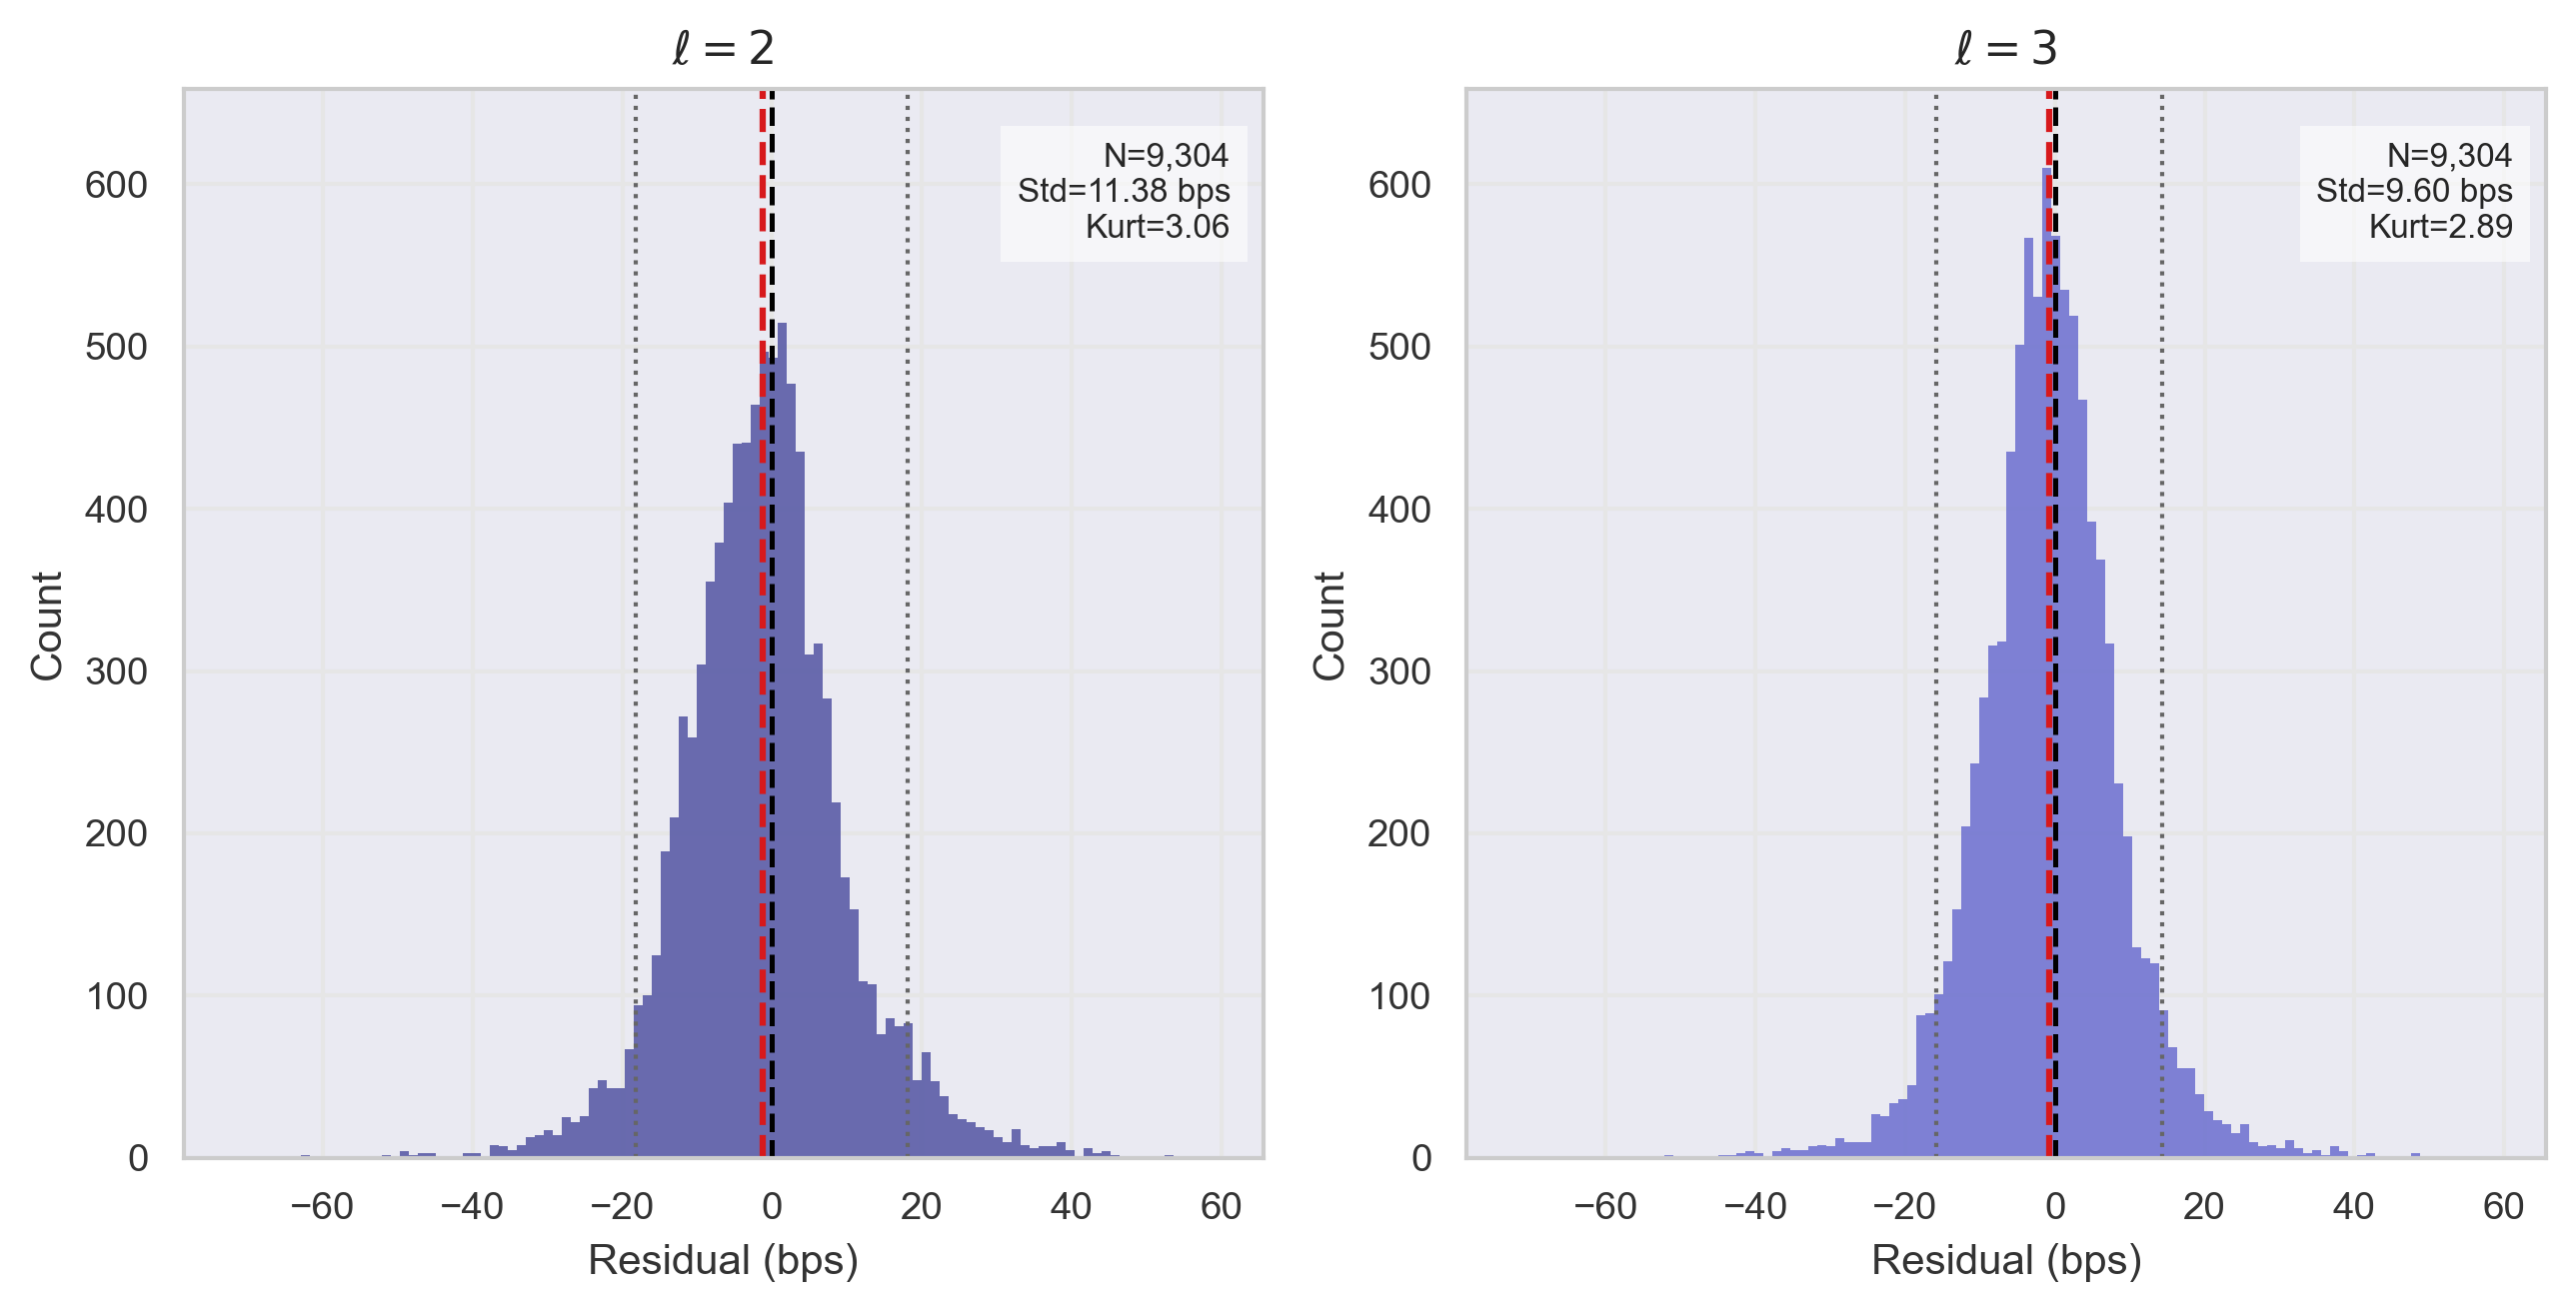
\includegraphics[width=0.85\textwidth]{Figures/thesis_results/AutoencoderPerformance/Q1d_residual_histograms_all_dims.png}
    \caption{Distribution of in-sample residuals (actual minus fitted) in basis points for
    $\ell \in \{1,2,3,4\}$ latent factors, pooled across all currencies and observation dates.
    Each panel corresponds to one latent dimension, coloured accordingly.
    The vertical dashed black line marks zero; the dashed red line marks the sample mean;
    the grey dotted lines mark the 5th and 95th percentiles. Sample size, standard deviation,
    and excess kurtosis are reported in the upper-right corner of each panel.}
    \label{fig:q1d_residual_histograms}
\end{figure}

%Q1d
\begin{figure}[htbp]
    \centering
    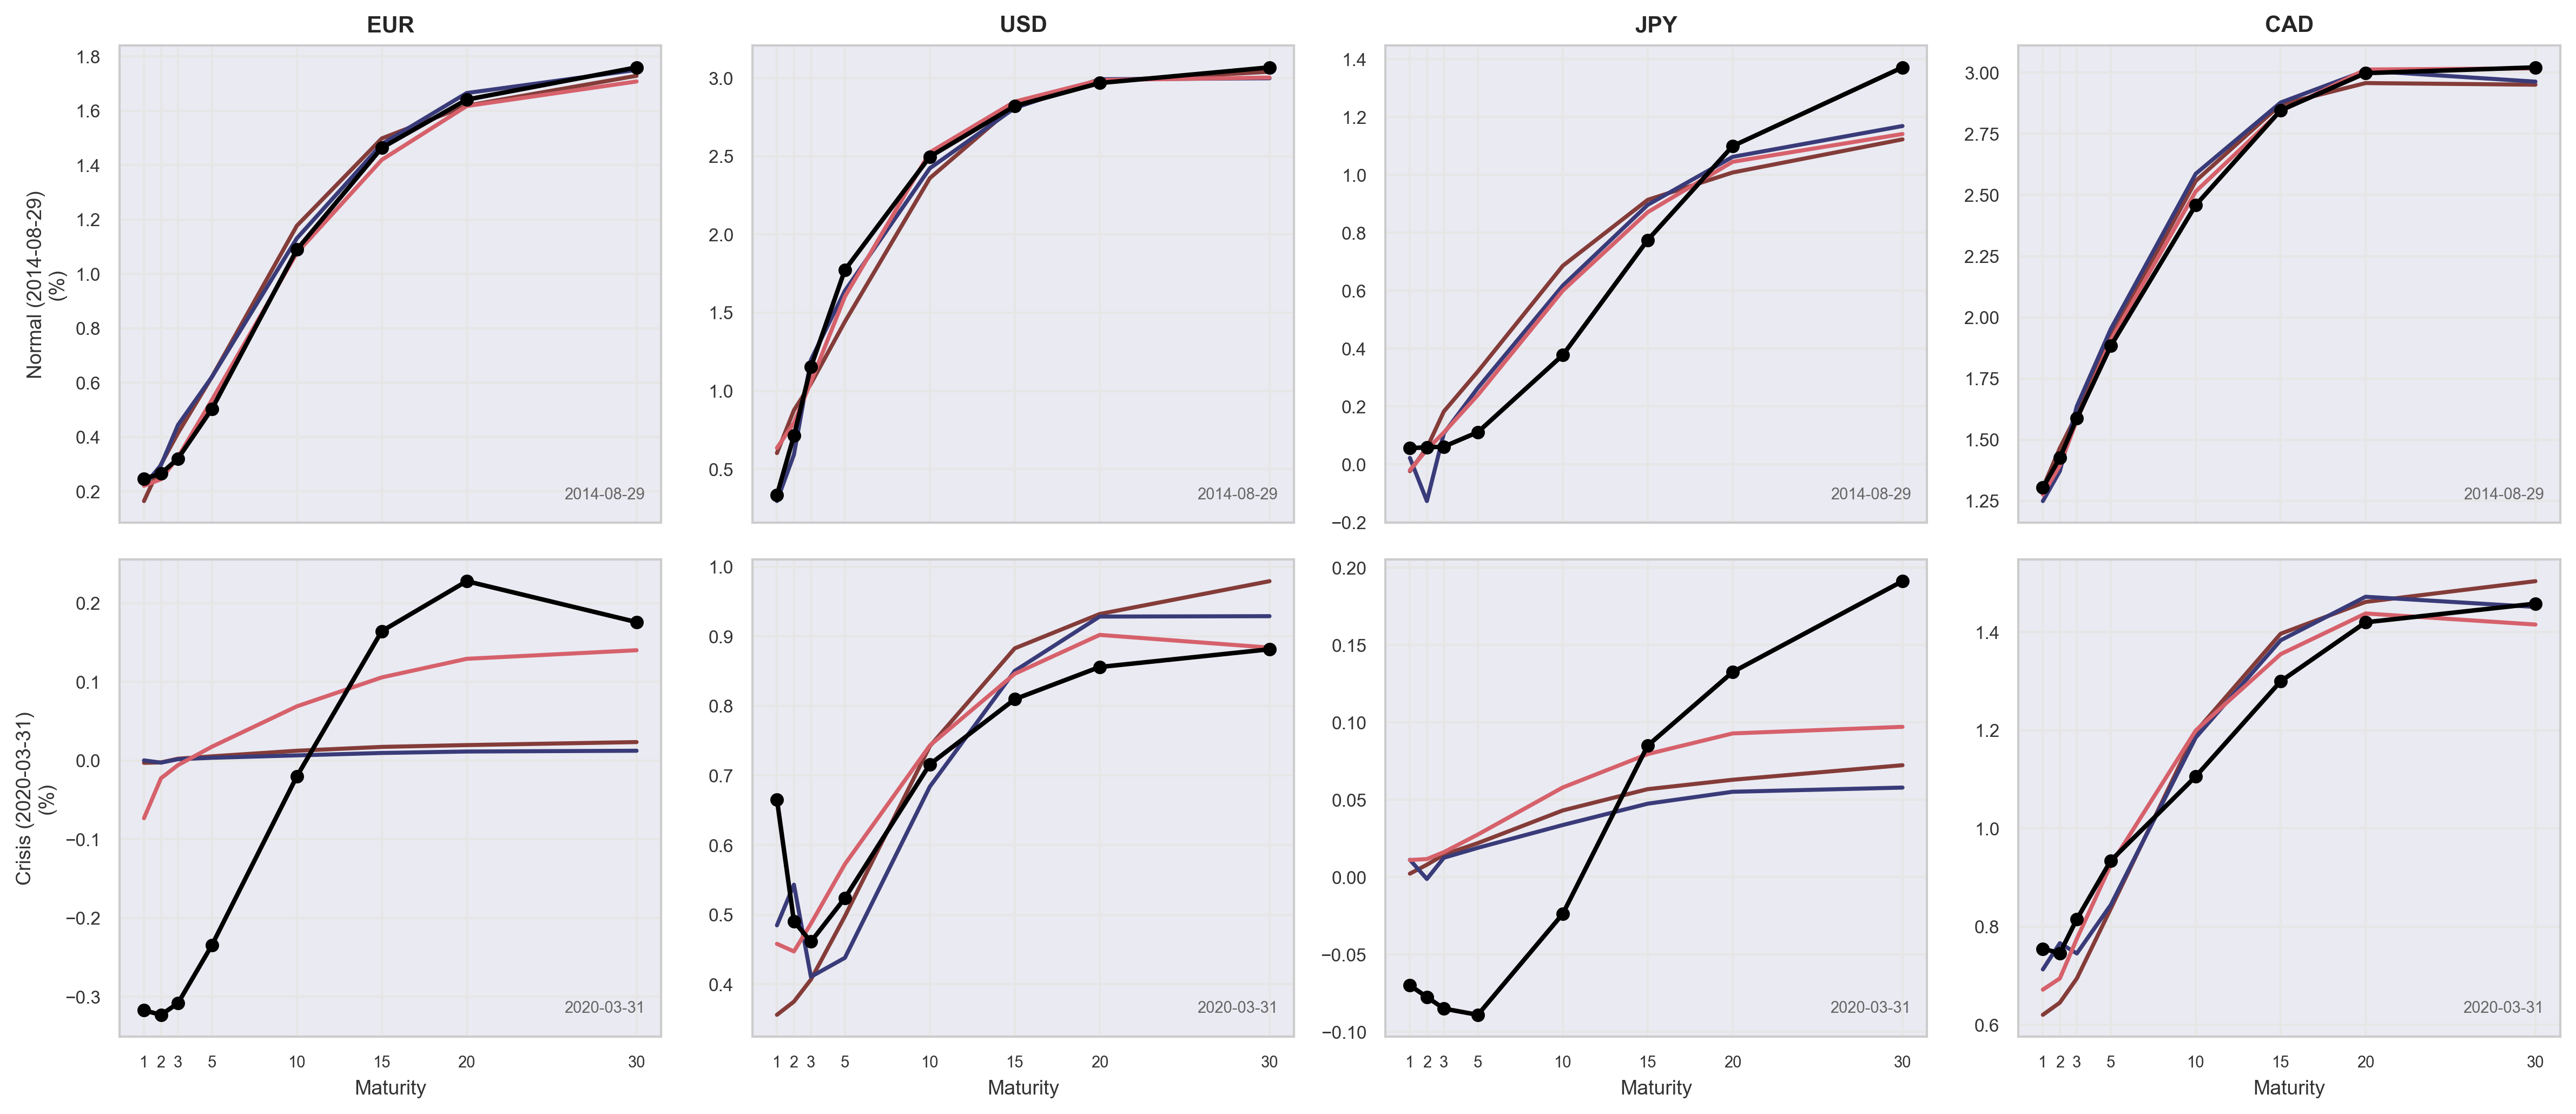
\includegraphics[width=\textwidth]{Figures/thesis_results/AutoencoderPerformance/Q1d_fitted_vs_actual_all_dims.png}
    \caption{In-sample fitted versus actual swap curves for latent dimensions
    $\ell \in \{2, 3, 4\}$ across three representative dates (columns): a normal market
    environment (2016-08-31), the Covid-19 stress episode (2020-03-31), and a low-rate
    regime (2019-06-30). Rows correspond to EUR and USD.
    The solid line with circles ({\color[HTML]{000000}\rule[0.5ex]{1em}{1.5pt}~$\circ$})
    denotes the observed swap rate.
    Reconstructions are shown for
    $\ell=2$ ({\color[HTML]{5254A3}\rule[0.5ex]{1em}{1.5pt}}, solid),
    $\ell=3$ ({\color[HTML]{6B6ECF}\rule[0.5ex]{1.2em}{1pt} \rule[0.5ex]{0.3em}{1pt}}, dashed), and
    $\ell=4$ ({\color[HTML]{9C9EDE}$\cdots$}, dotted).
    The x-axis shows tenor in years. The exact observation date is printed in
    the lower-right corner of each panel.}
    \label{fig:q1d_fitted_vs_actual_all_dims}
\end{figure}







% ─────────────────────────────────────────────────────────────
\section{Question 2}
% ─────────────────────────────────────────────────────────────

% ── Q2a ──────────────────────────────────────────────────────────────────────
\begin{table}[h!]
\centering
{\small
\pgfplotstableread[col sep=comma]{Figures/thesis_results/AutoencoderPerformance/Q2a_IS_vs_OOS_all_dims.csv}\datqtwoa
\resizebox{\textwidth}{!}{%
\pgfplotstabletypeset[
  columns={Split, Model, AUD, CAD, DKK, EUR, JPY, NOK, SEK, GBP, USD, Average},
  columns/Split/.style={string type, column type=l},
  columns/Model/.style={string type, column type=l},
  columns/AUD/.style={column type=r, fixed, precision=2, fixed zerofill},
  columns/CAD/.style={column type=r, fixed, precision=2, fixed zerofill},
  columns/DKK/.style={column type=r, fixed, precision=2, fixed zerofill},
  columns/EUR/.style={column type=r, fixed, precision=2, fixed zerofill},
  columns/JPY/.style={column type=r, fixed, precision=2, fixed zerofill},
  columns/NOK/.style={column type=r, fixed, precision=2, fixed zerofill},
  columns/SEK/.style={column type=r, fixed, precision=2, fixed zerofill},
  columns/GBP/.style={column type=r, fixed, precision=2, fixed zerofill},
  columns/USD/.style={column type=r, fixed, precision=2, fixed zerofill},
  columns/Average/.style={column name={\textbf{Avg.}}, column type=r, fixed, precision=2, fixed zerofill},
  every head row/.style={before row=\toprule, after row=\midrule},
  every last row/.style={after row=\bottomrule},
]{\datqtwoa}}
}
\caption{In-sample and out-of-sample RMSE (bps) per currency across latent dimensions.
IS: 2004--2020, OOS: 2021--2022.}
\label{tab:q2a_is_oos_rmse}
\end{table}


% Q2b
\begin{figure}[H]
    \centering
    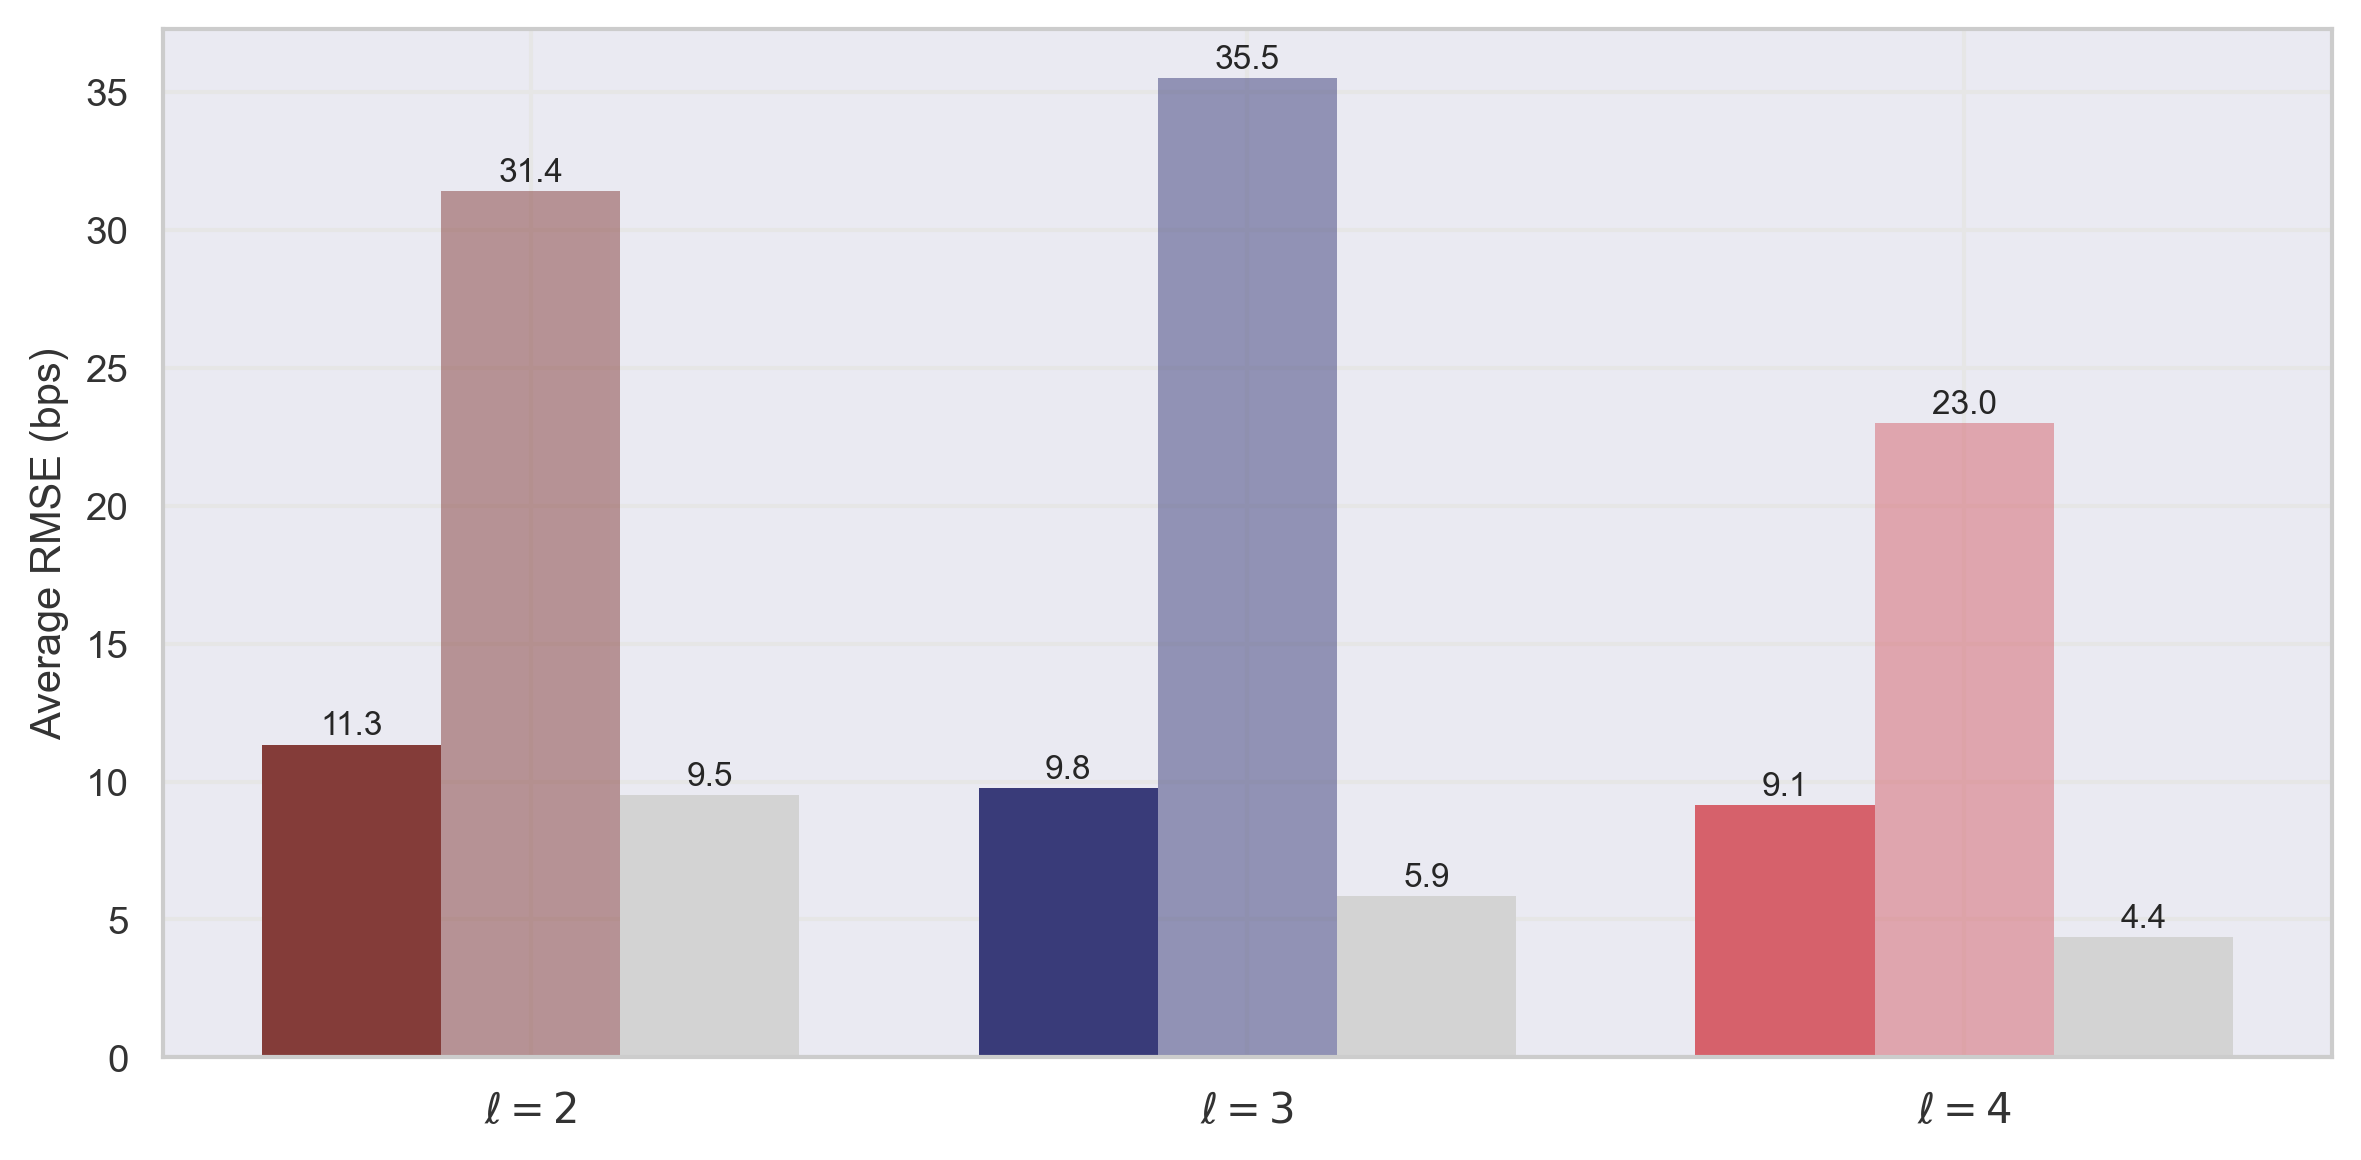
\includegraphics[width=0.75\textwidth]{Figures/thesis_results/AutoencoderPerformance/Q2b_rolling_oos_vs_dim.png}
    \caption{Rolling out-of-sample RMSE (bps) by latent dimension $\ell$,
    averaged across 34 rolling windows (3-year train, 3-month test).}
    \label{fig:Q2b}
\end{figure}



% ─────────────────────────────────────────────────────────────
\section{Question 3}
% ─────────────────────────────────────────────────────────────

% Q3a
\begin{table}[H]
\centering
\begin{tabular}{lrrrrrrrrrrr}
\toprule
 & AUD & CAD & DKK & EUR & JPY & NOK & SEK & GBP & USD & \textbf{Avg} \\
\midrule
Seed 0 & 11.79 & 10.83 & 14.46 & 24.11 & 8.37 & 16.68 & 12.92 & 12.70 & 13.72 & 13.95 \\
Seed 1 & 11.51 & 12.36 & 12.57 & 22.97 & 7.74 & 10.64 & 10.23 & 13.08 & 12.54 & 12.63 \\
Seed 2 & 9.55  & 8.99  & 10.20 & 18.31 & 7.43 & 11.18 & 8.61  & 10.06 & 9.46  & 10.42 \\
Seed 3 & 8.34  & 9.15  & 9.77  & 15.59 & 9.26 & 9.19  & 6.52  & 7.33  & 10.94 & \textbf{9.57}  \\
Seed 4 & \multicolumn{10}{c}{\textit{diverged (1663 bps) --- excluded}} \\
Seed 5 & 9.11  & 9.58  & 17.55 & 23.15 & 4.95 & 13.80 & 12.44 & 22.67 & 13.61 & 14.10 \\
Seed 6 & 14.20 & 9.33  & 23.60 & 28.78 & 4.86 & 19.26 & 17.98 & 26.12 & 14.59 & 17.64 \\
Seed 7 & \multicolumn{10}{c}{\textit{diverged (NaN) --- excluded}} \\
Seed 8 & 9.23  & 10.64 & 11.48 & 22.68 & 8.68 & 11.79 & 9.82  & 9.32  & 12.37 & 11.78 \\
Seed 9 & 11.30 & 9.00  & 12.06 & 21.37 & 8.30 & 11.84 & 10.07 & 10.91 & 10.59 & 11.72 \\
\midrule
\textbf{Mean (valid)} & & & & & & & & & & \textbf{12.72} \\
\bottomrule
\end{tabular}
\caption{Out-of-sample RMSE (bps) per random seed for $\ell=3$.
Seeds 4 and 7 diverged and are excluded from the mean.}
\label{tab:Q3a}
\end{table}



% Q3b
\begin{figure}[H]
    \centering
    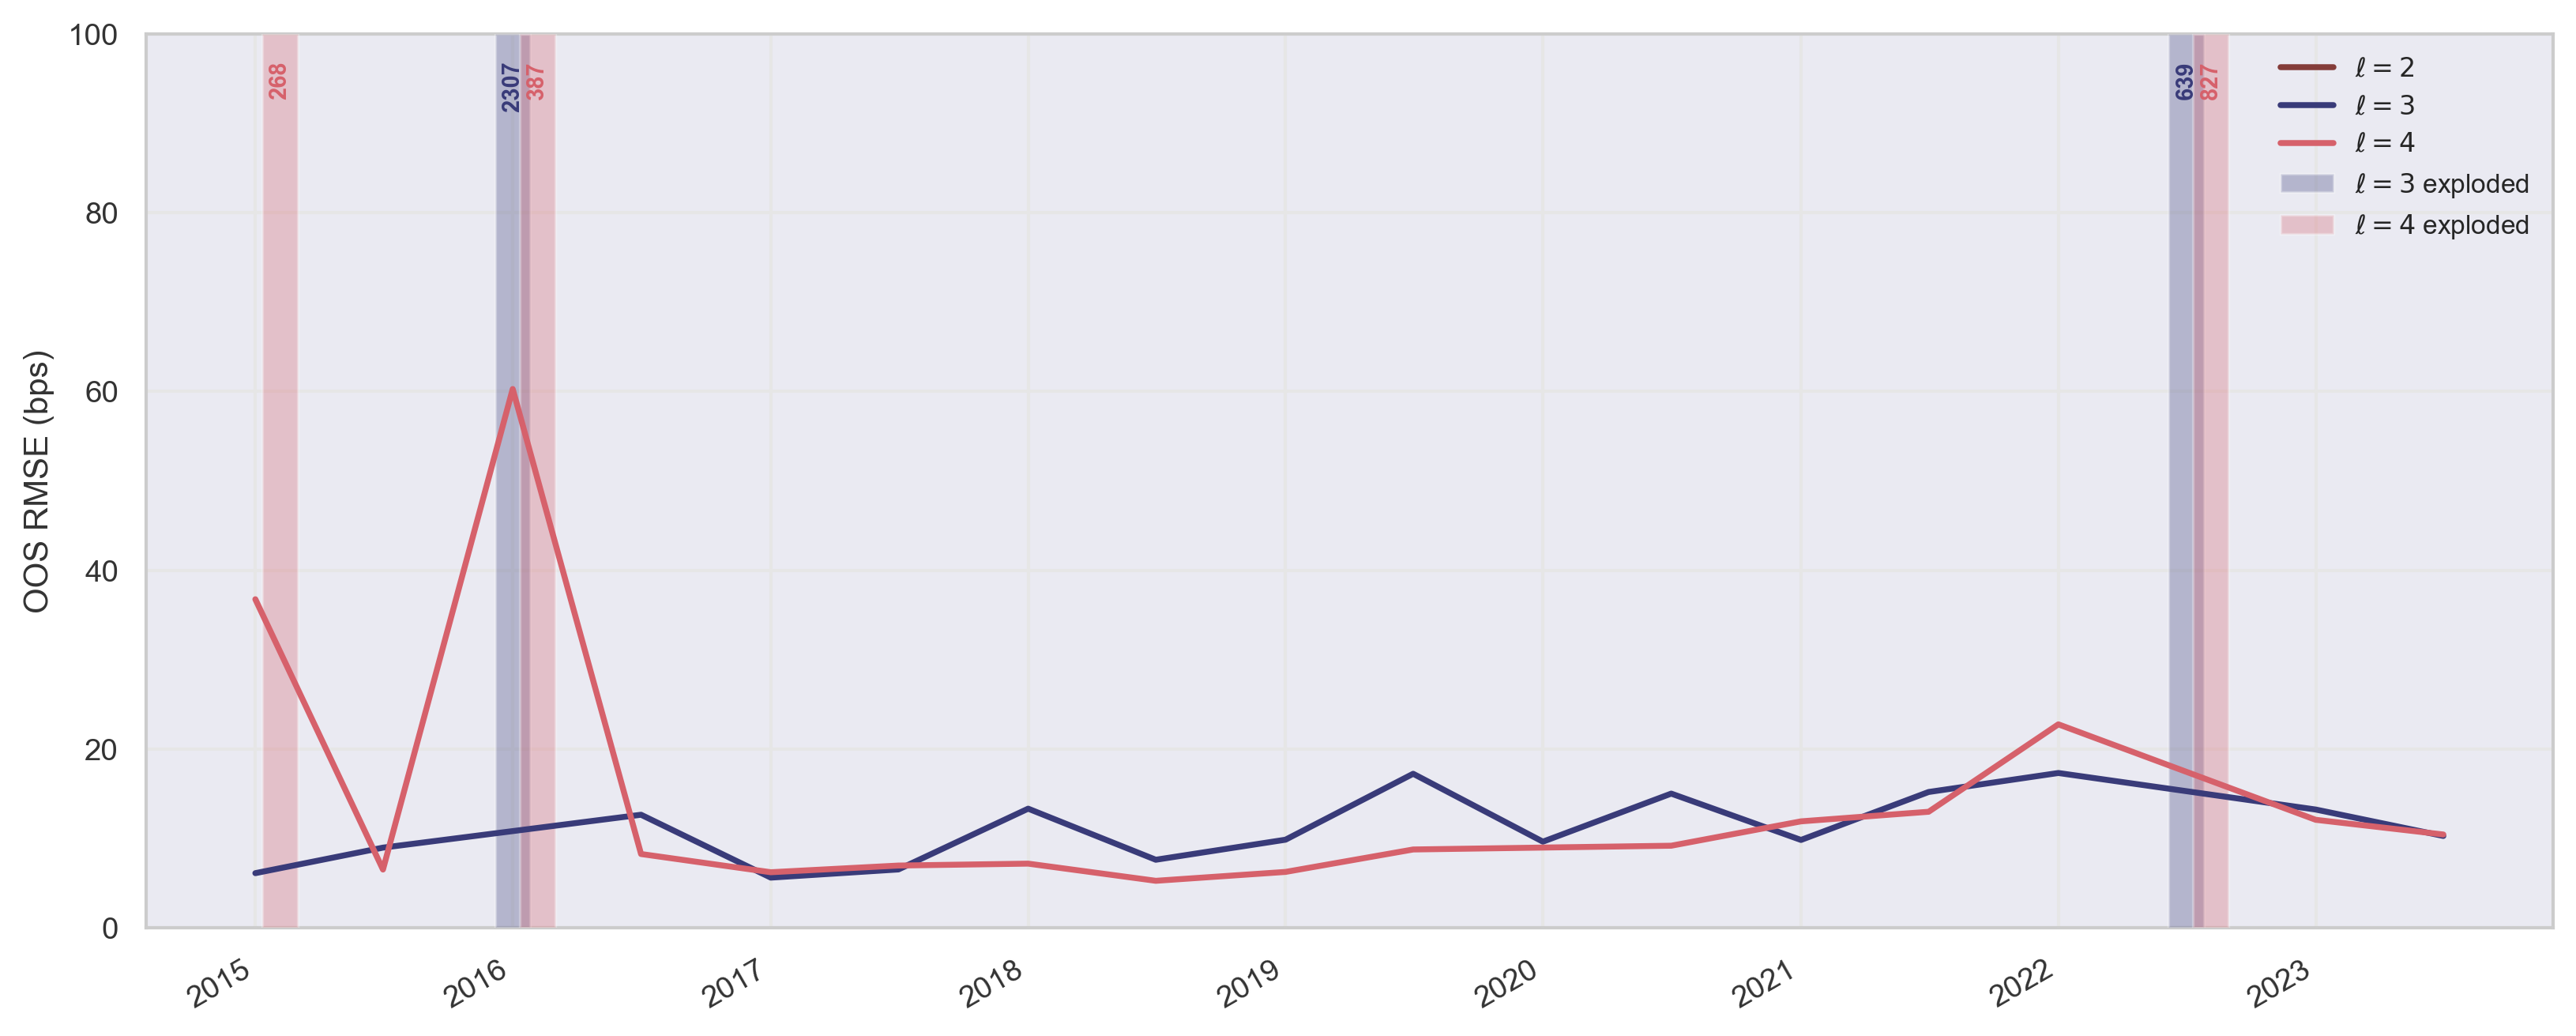
\includegraphics[width=0.9\textwidth]{Figures/thesis_results/AutoencoderPerformance/Q3b_rolling_rmse_over_time.png}
    \caption{Rolling out-of-sample RMSE over time for $\ell=3$,
    showing variation across rolling windows.}
    \label{fig:Q3b}
\end{figure}

% ─────────────────────────────────────────────────────────────
\section{Question 4}
% ─────────────────────────────────────────────────────────────

% Q4a

% ── Q4a ──────────────────────────────────────────────────────────────────────
\begin{table}[H]
\centering
{\small
\pgfplotstableread[col sep=comma]{Figures/thesis_results/AutoencoderPerformance/Q4a_AE_vs_Kalman_OOS.csv}\datqfoura
\resizebox{\textwidth}{!}{%
\pgfplotstabletypeset[
  columns={index, AUD, CAD, DKK, EUR, JPY, NOK, SEK, GBP, USD, Average},
  columns/index/.style={column name={Model}, string type, column type=l},
  columns/AUD/.style={column type=r, fixed, precision=2, fixed zerofill},
  columns/CAD/.style={column type=r, fixed, precision=2, fixed zerofill},
  columns/DKK/.style={column type=r, fixed, precision=2, fixed zerofill},
  columns/EUR/.style={column type=r, fixed, precision=2, fixed zerofill},
  columns/JPY/.style={column type=r, fixed, precision=2, fixed zerofill},
  columns/NOK/.style={column type=r, fixed, precision=2, fixed zerofill},
  columns/SEK/.style={column type=r, fixed, precision=2, fixed zerofill},
  columns/GBP/.style={column type=r, fixed, precision=2, fixed zerofill},
  columns/USD/.style={column type=r, fixed, precision=2, fixed zerofill},
  columns/Average/.style={column name={\textbf{Avg}}, column type=r, fixed, precision=2, fixed zerofill},
  every head row/.style={before row=\toprule, after row=\midrule},
  every row no 2/.style={before row=\midrule},
  every row no 4/.style={before row=\midrule},
  every row no 6/.style={before row=\midrule},
  every last row/.style={after row=\bottomrule},
]{\datqfoura}}
}
\caption{Out-of-sample RMSE (bps) per currency for the autoencoder and EKF DNS benchmarks,
grouped by number of latent factors $\ell$ (2021--2022 test period).}
\label{tab:Q4a}
\end{table}








% Q4c
\begin{figure}[H]
    \centering
    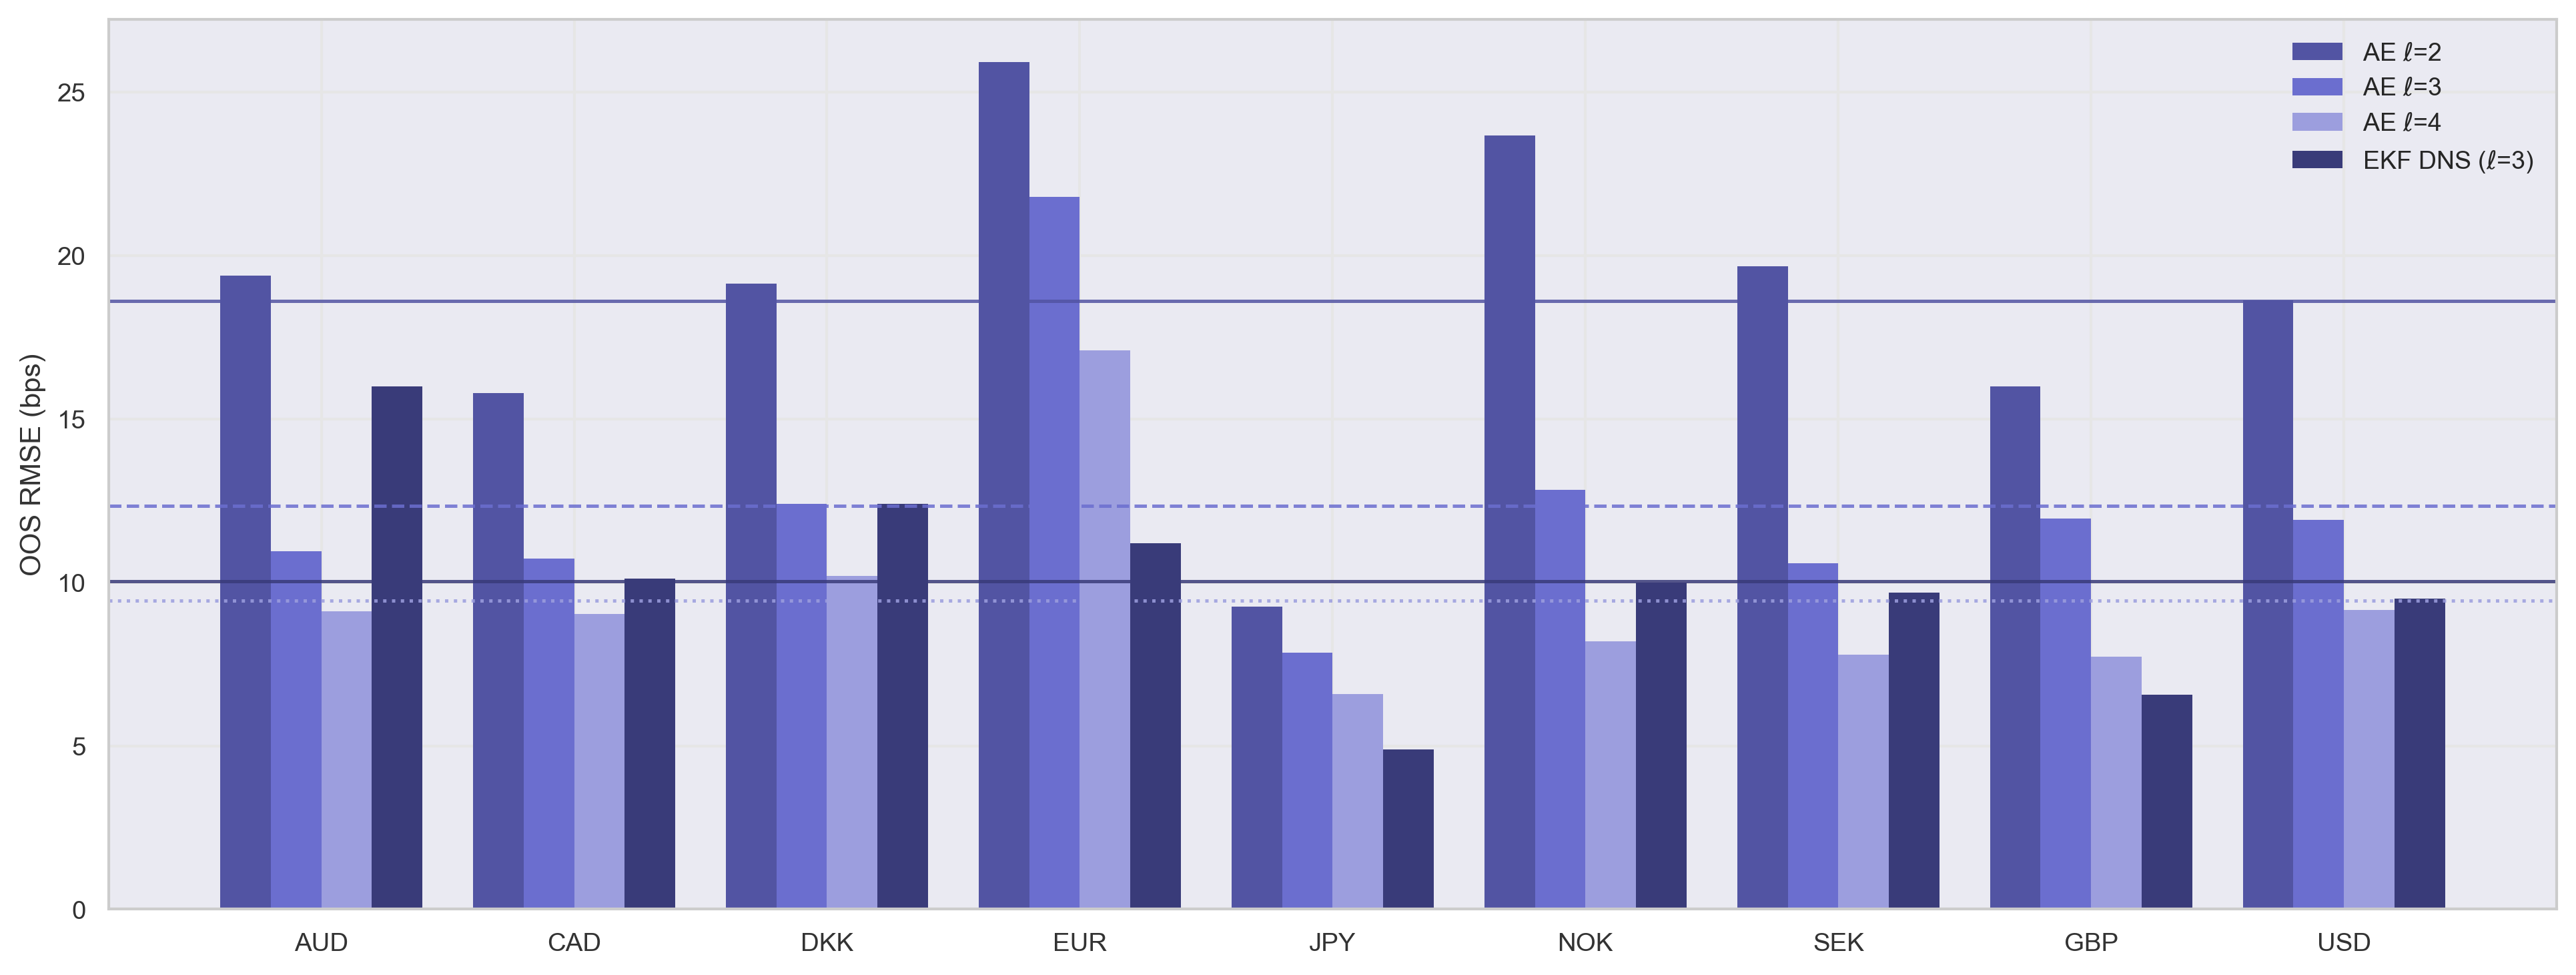
\includegraphics[width=1.0\textwidth]{Figures/thesis_results/AutoencoderPerformance/Q4c_per_currency_bar_chart_all_dims.png}
    \caption{Out-of-sample RMSE (bps) per currency for autoencoder
    dimensions $\ell=2,3,4$ and EKF DNS 3-factor benchmark.}
    \label{fig:Q4c}
\end{figure}

% ─────────────────────────────────────────────────────────────
\section{Question 5}
% ─────────────────────────────────────────────────────────────

\begin{figure}[H]
    \centering
    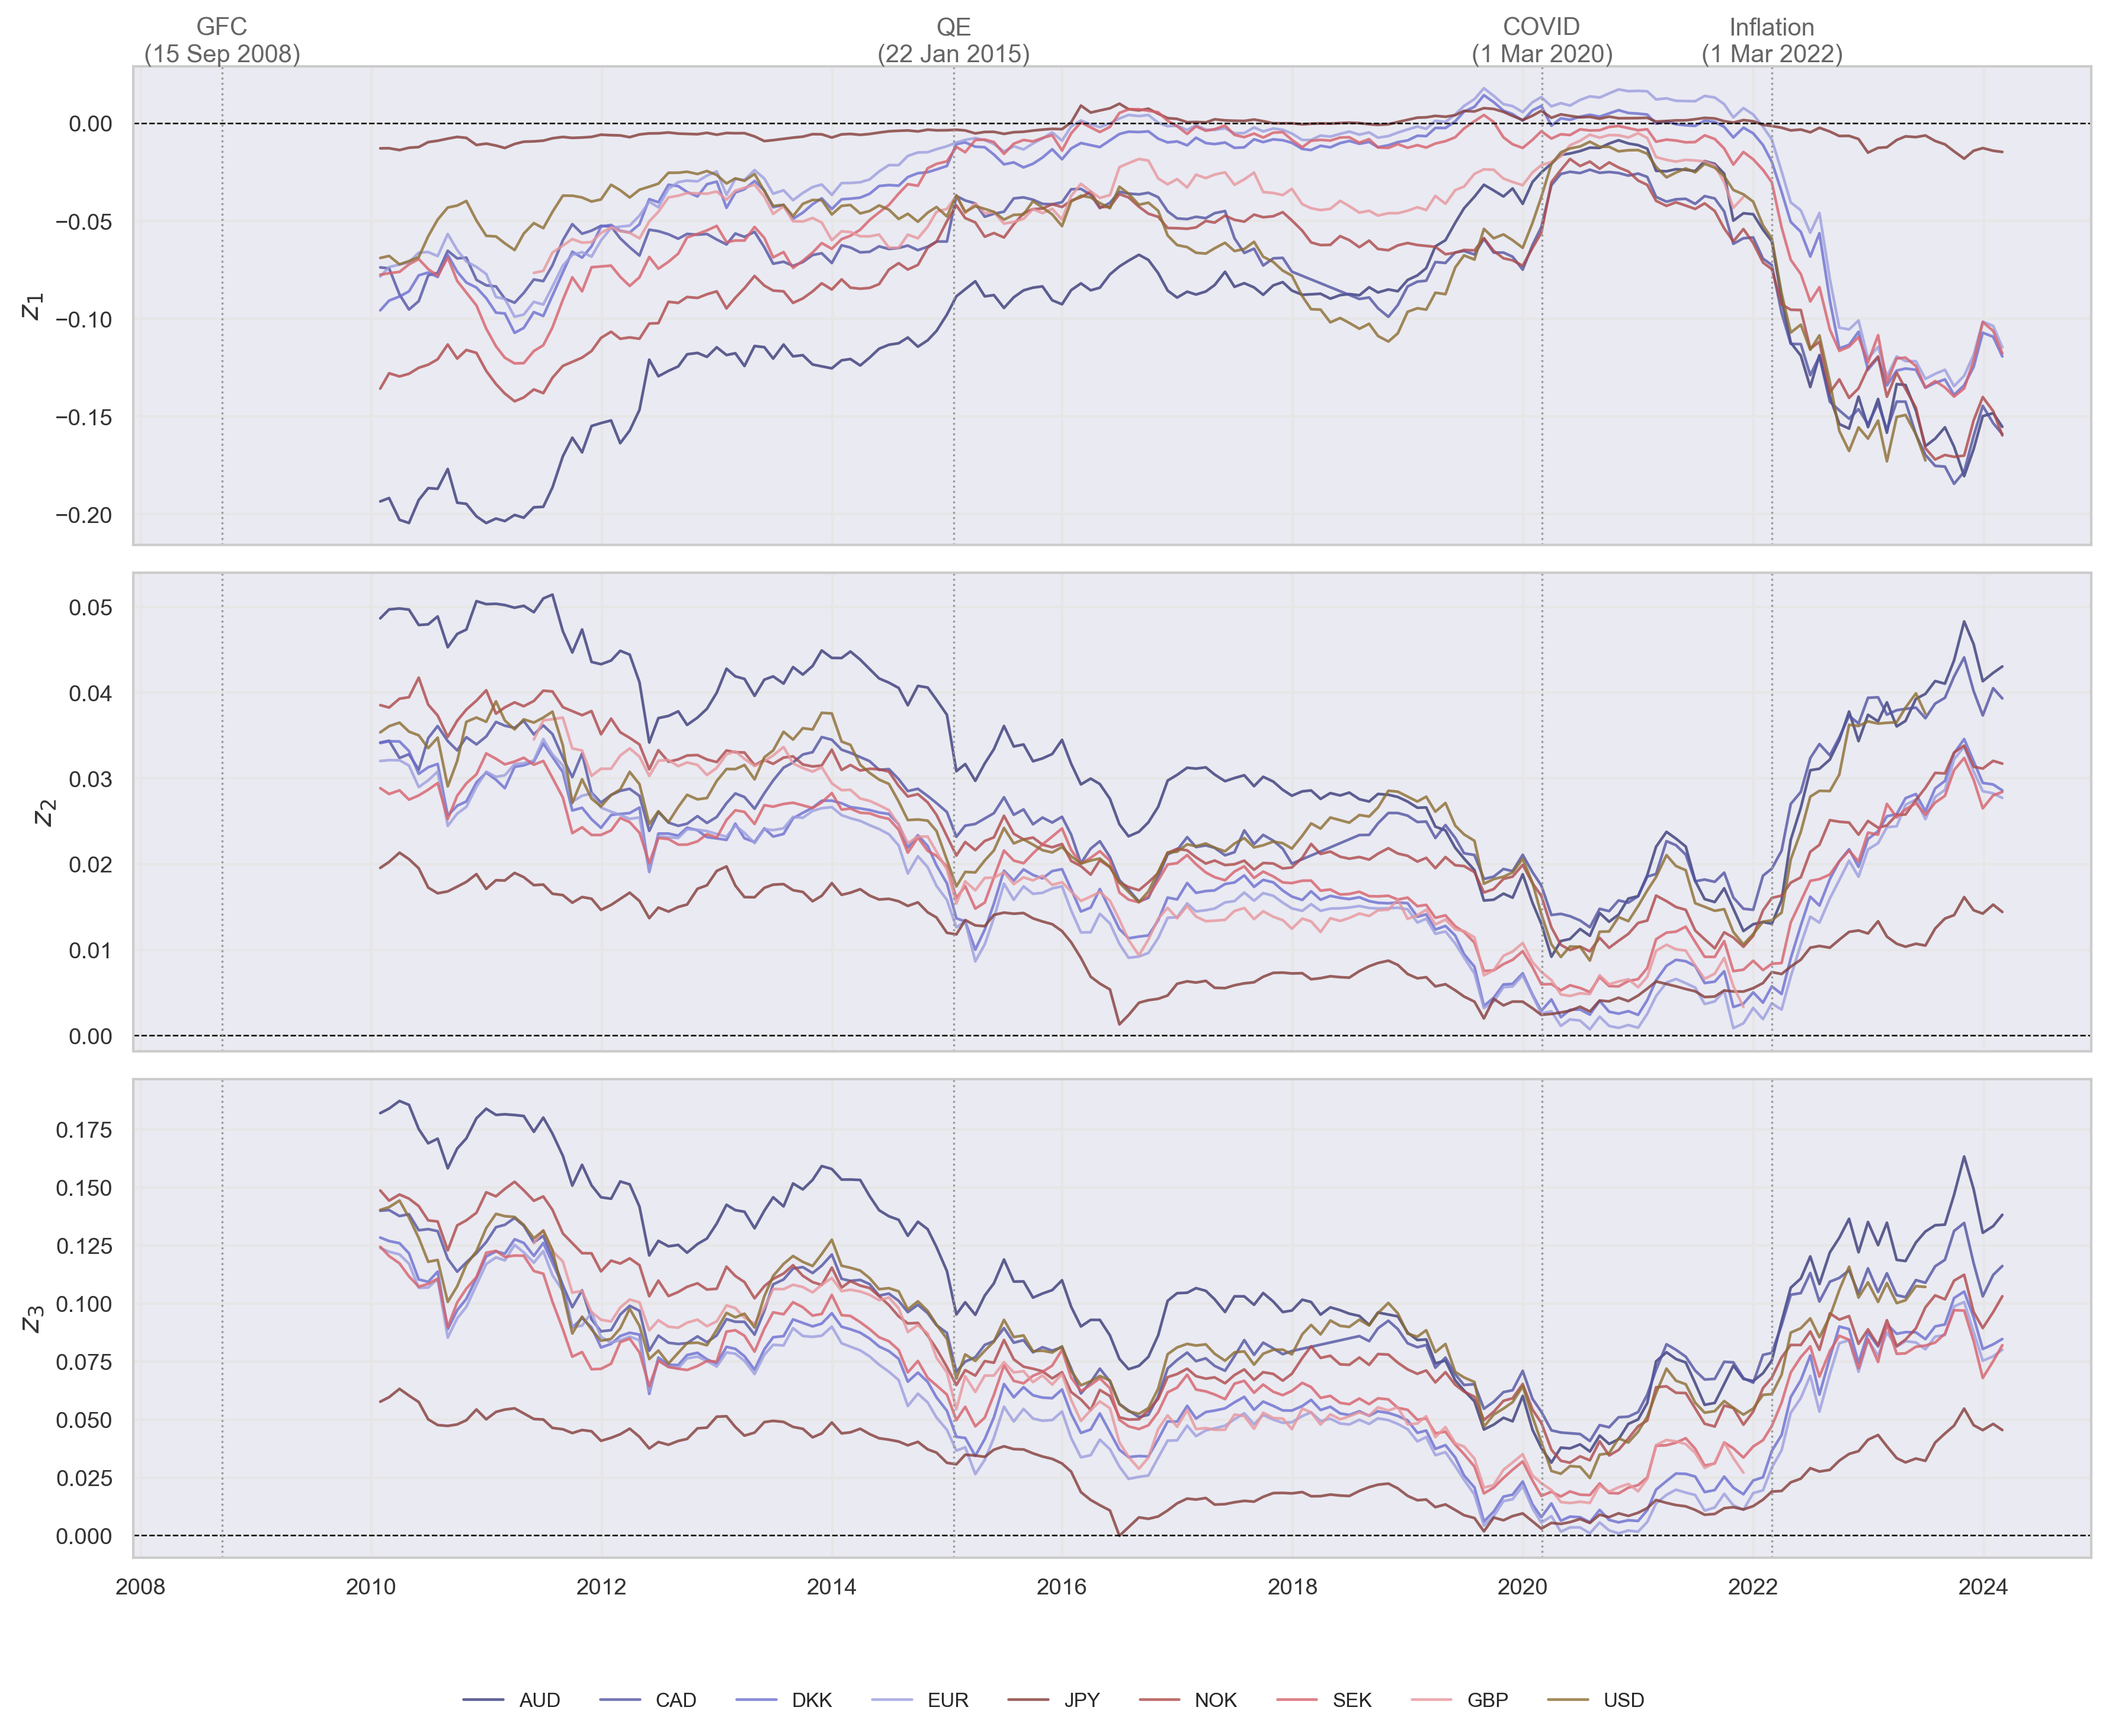
\includegraphics[width=\textwidth]{Figures/thesis_results/AutoencoderPerformance/Q5a_latent_factors_over_time.png}
    \caption{Latent factors $z_1, z_2, z_3$ over the training period
    (2004--2020) for $\ell=3$, with key market events annotated.}
    \label{fig:Q5a}
\end{figure}


\begin{figure}[htbp]
    \centering
    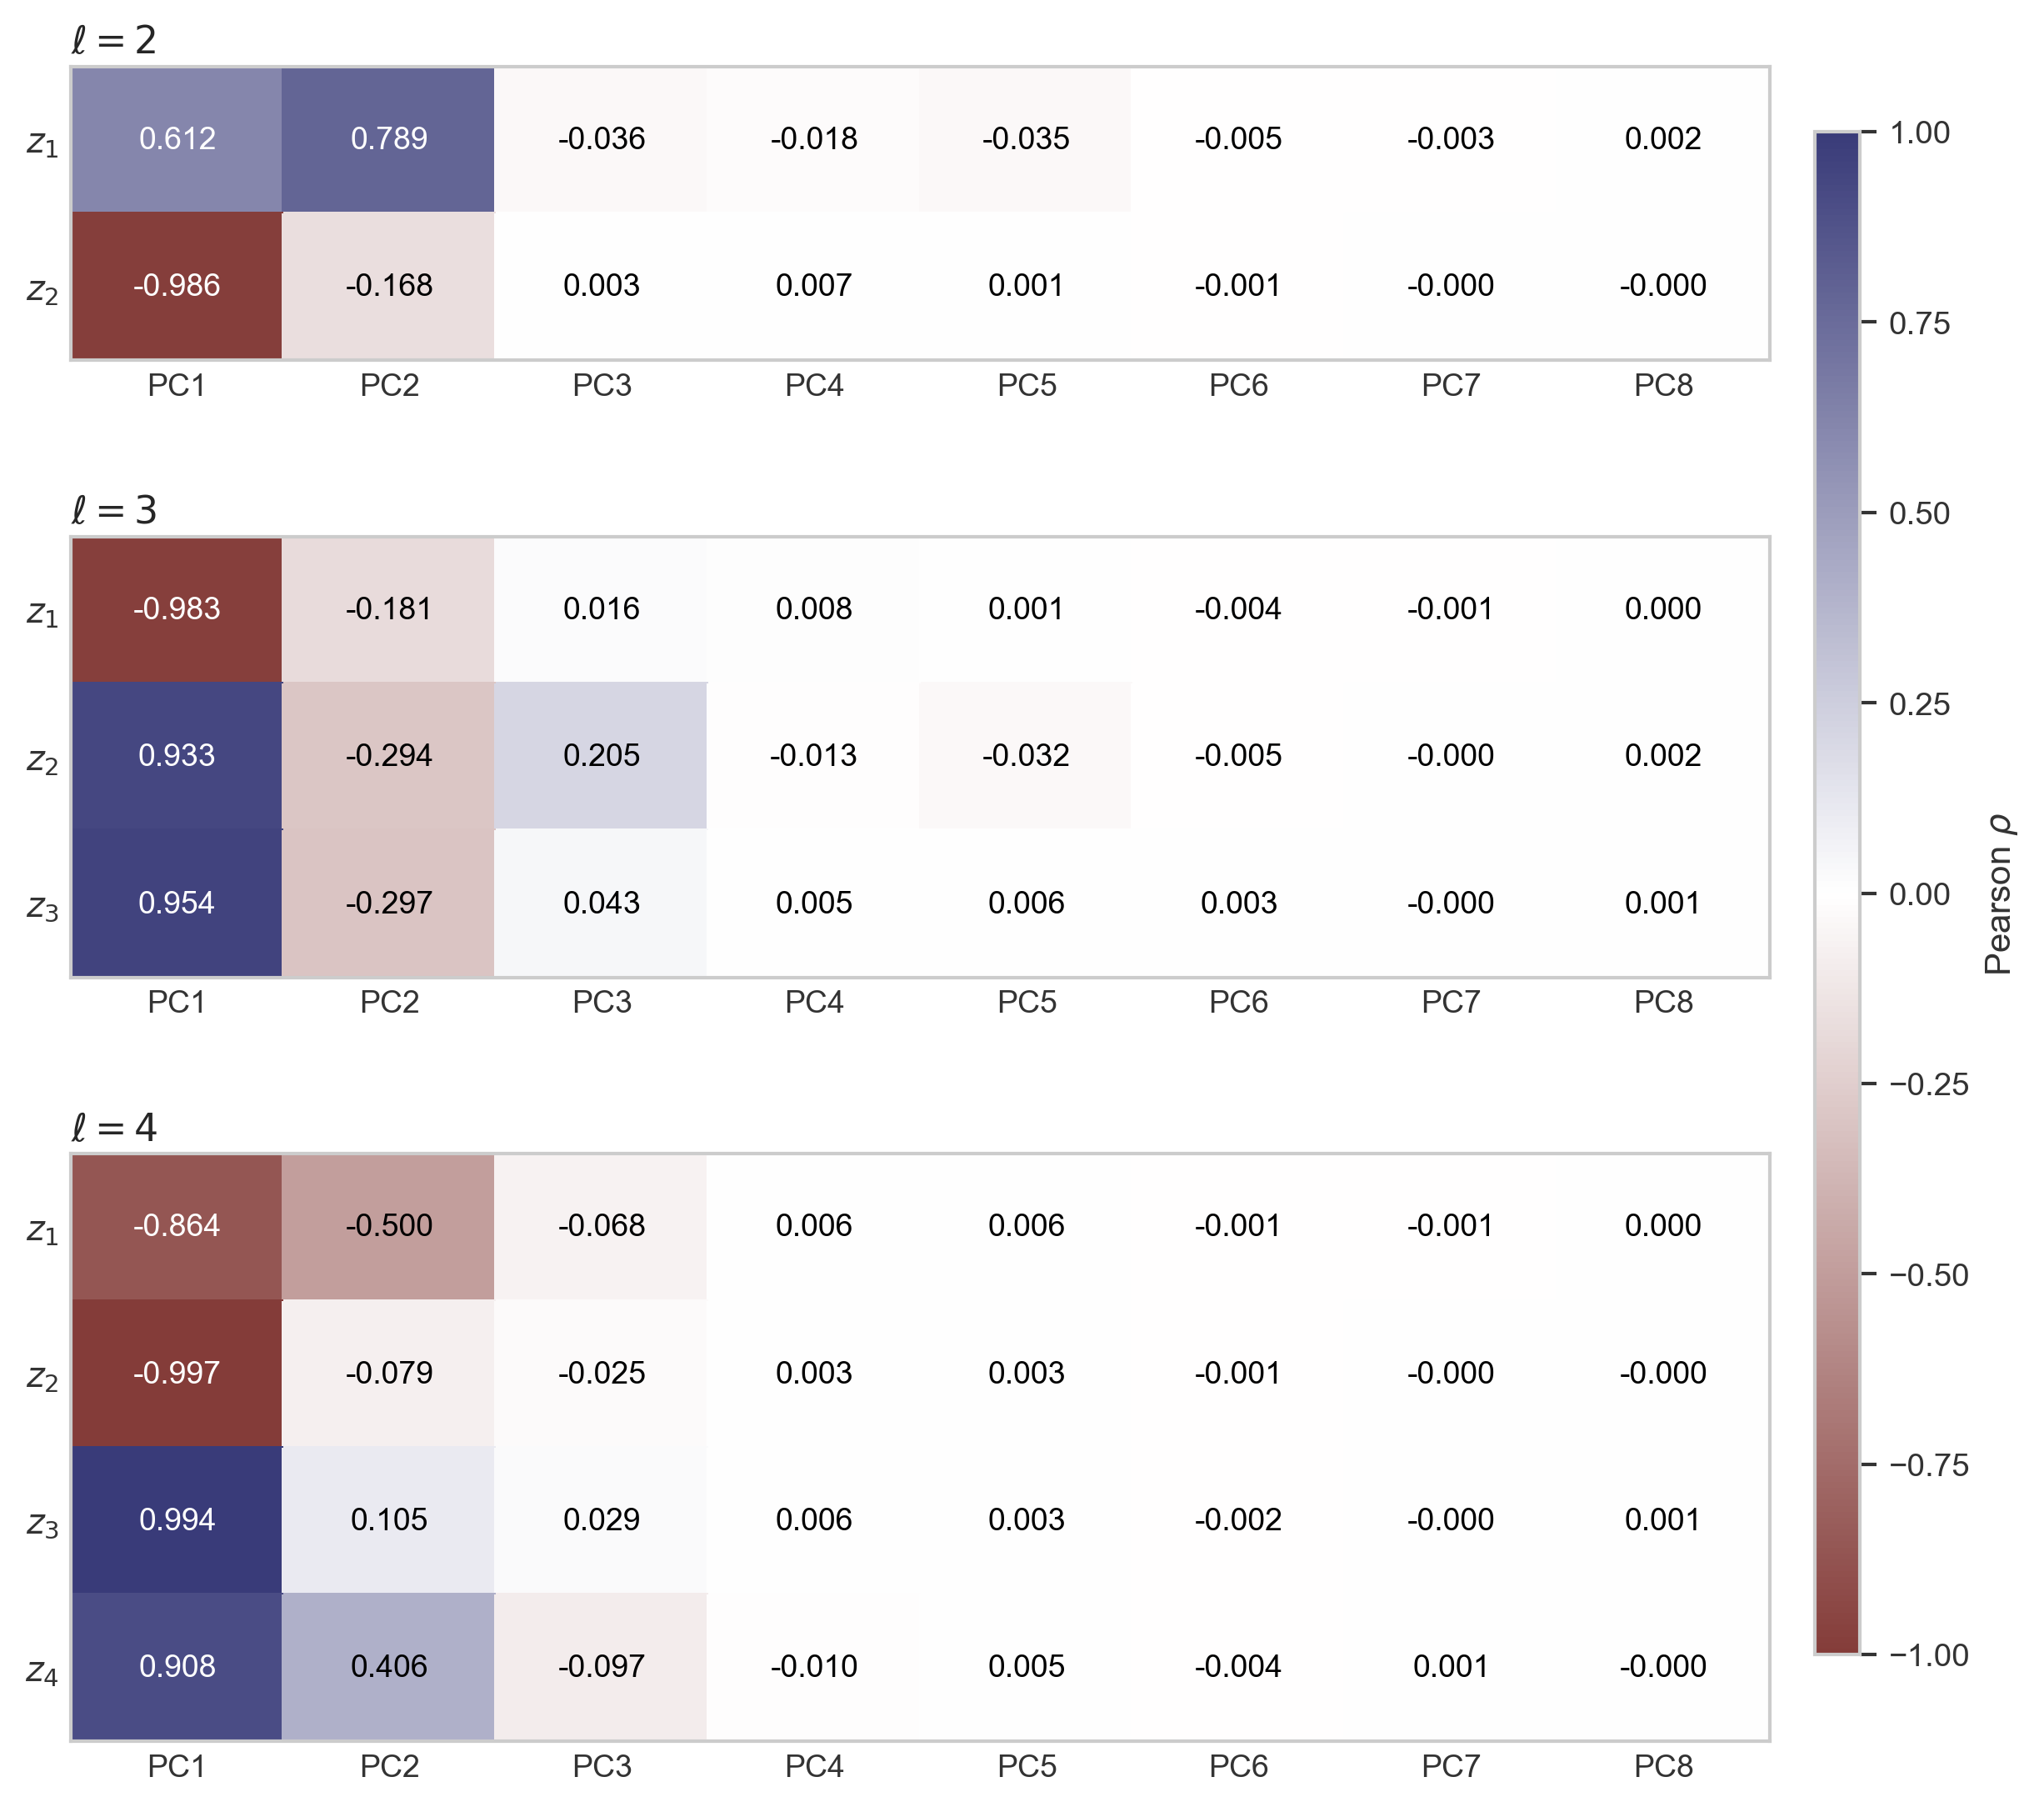
\includegraphics[width=\textwidth]{Figures/thesis_results/AutoencoderPerformance/Q5b_factor_correlation_heatmap.png}
    \caption{Pearson correlation between each latent factor $z_k$ and the level, slope, and curvature of the swap curve, for $\ell \in \{2, 3, 4\}$. Blue indicates positive correlation, red indicates negative correlation. Correlations are computed on the in-sample training observations.}
    \label{fig:q5b_factor_correlation_heatmap}
\end{figure}



% ─────────────────────────────────────────────────────────────
\section{Question 6}
% ─────────────────────────────────────────────────────────────


%Q6a
\begin{figure}[H]
    \centering
    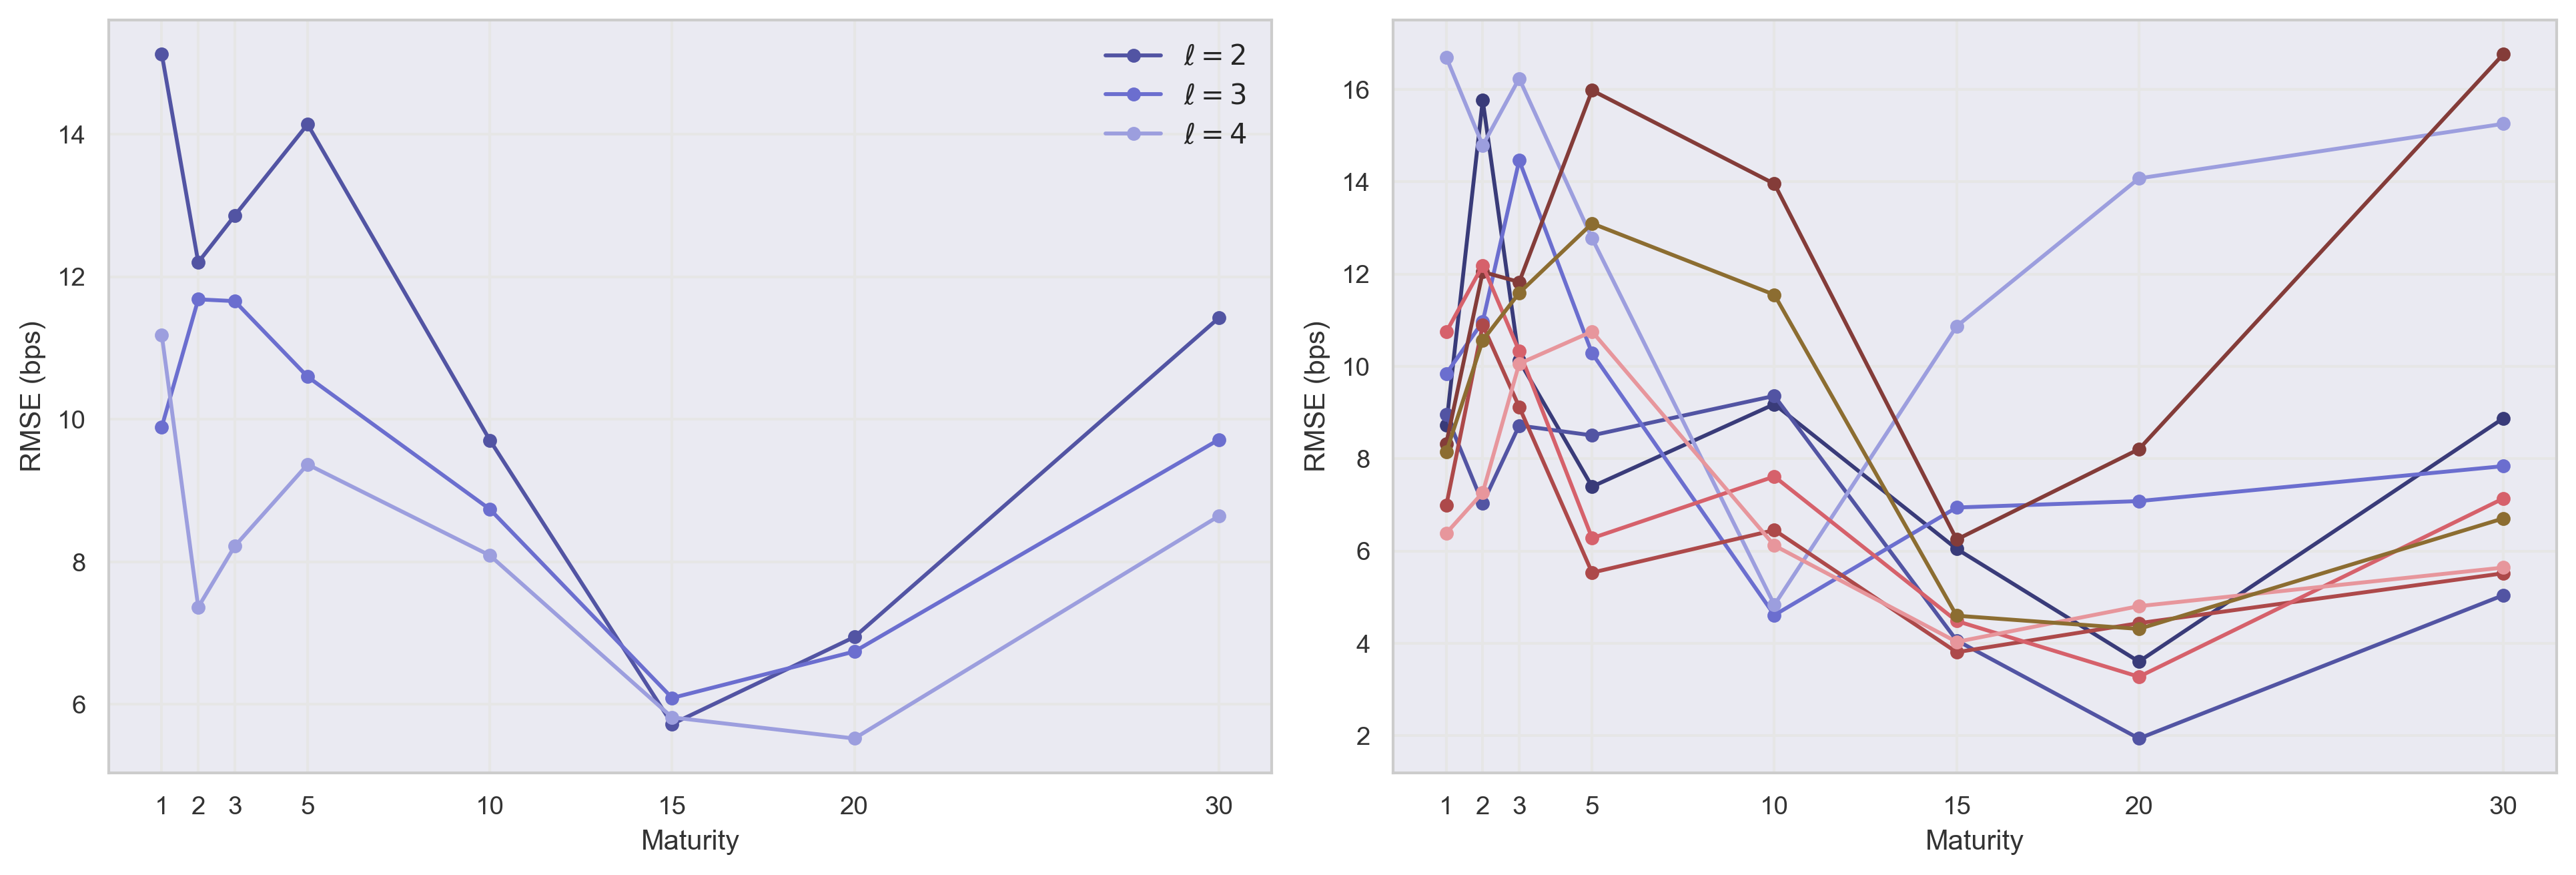
\includegraphics[width=1.0\textwidth]{Figures/thesis_results/AutoencoderPerformance/Q6a_rmse_by_tenor.png}
    \caption{In-sample RMSE (bps) by tenor for $\ell=3$,
    averaged across currencies and dates in the training set.}
    \label{fig:Q6a}
\end{figure}


%Q6b
\begin{figure}[H]
    \centering
    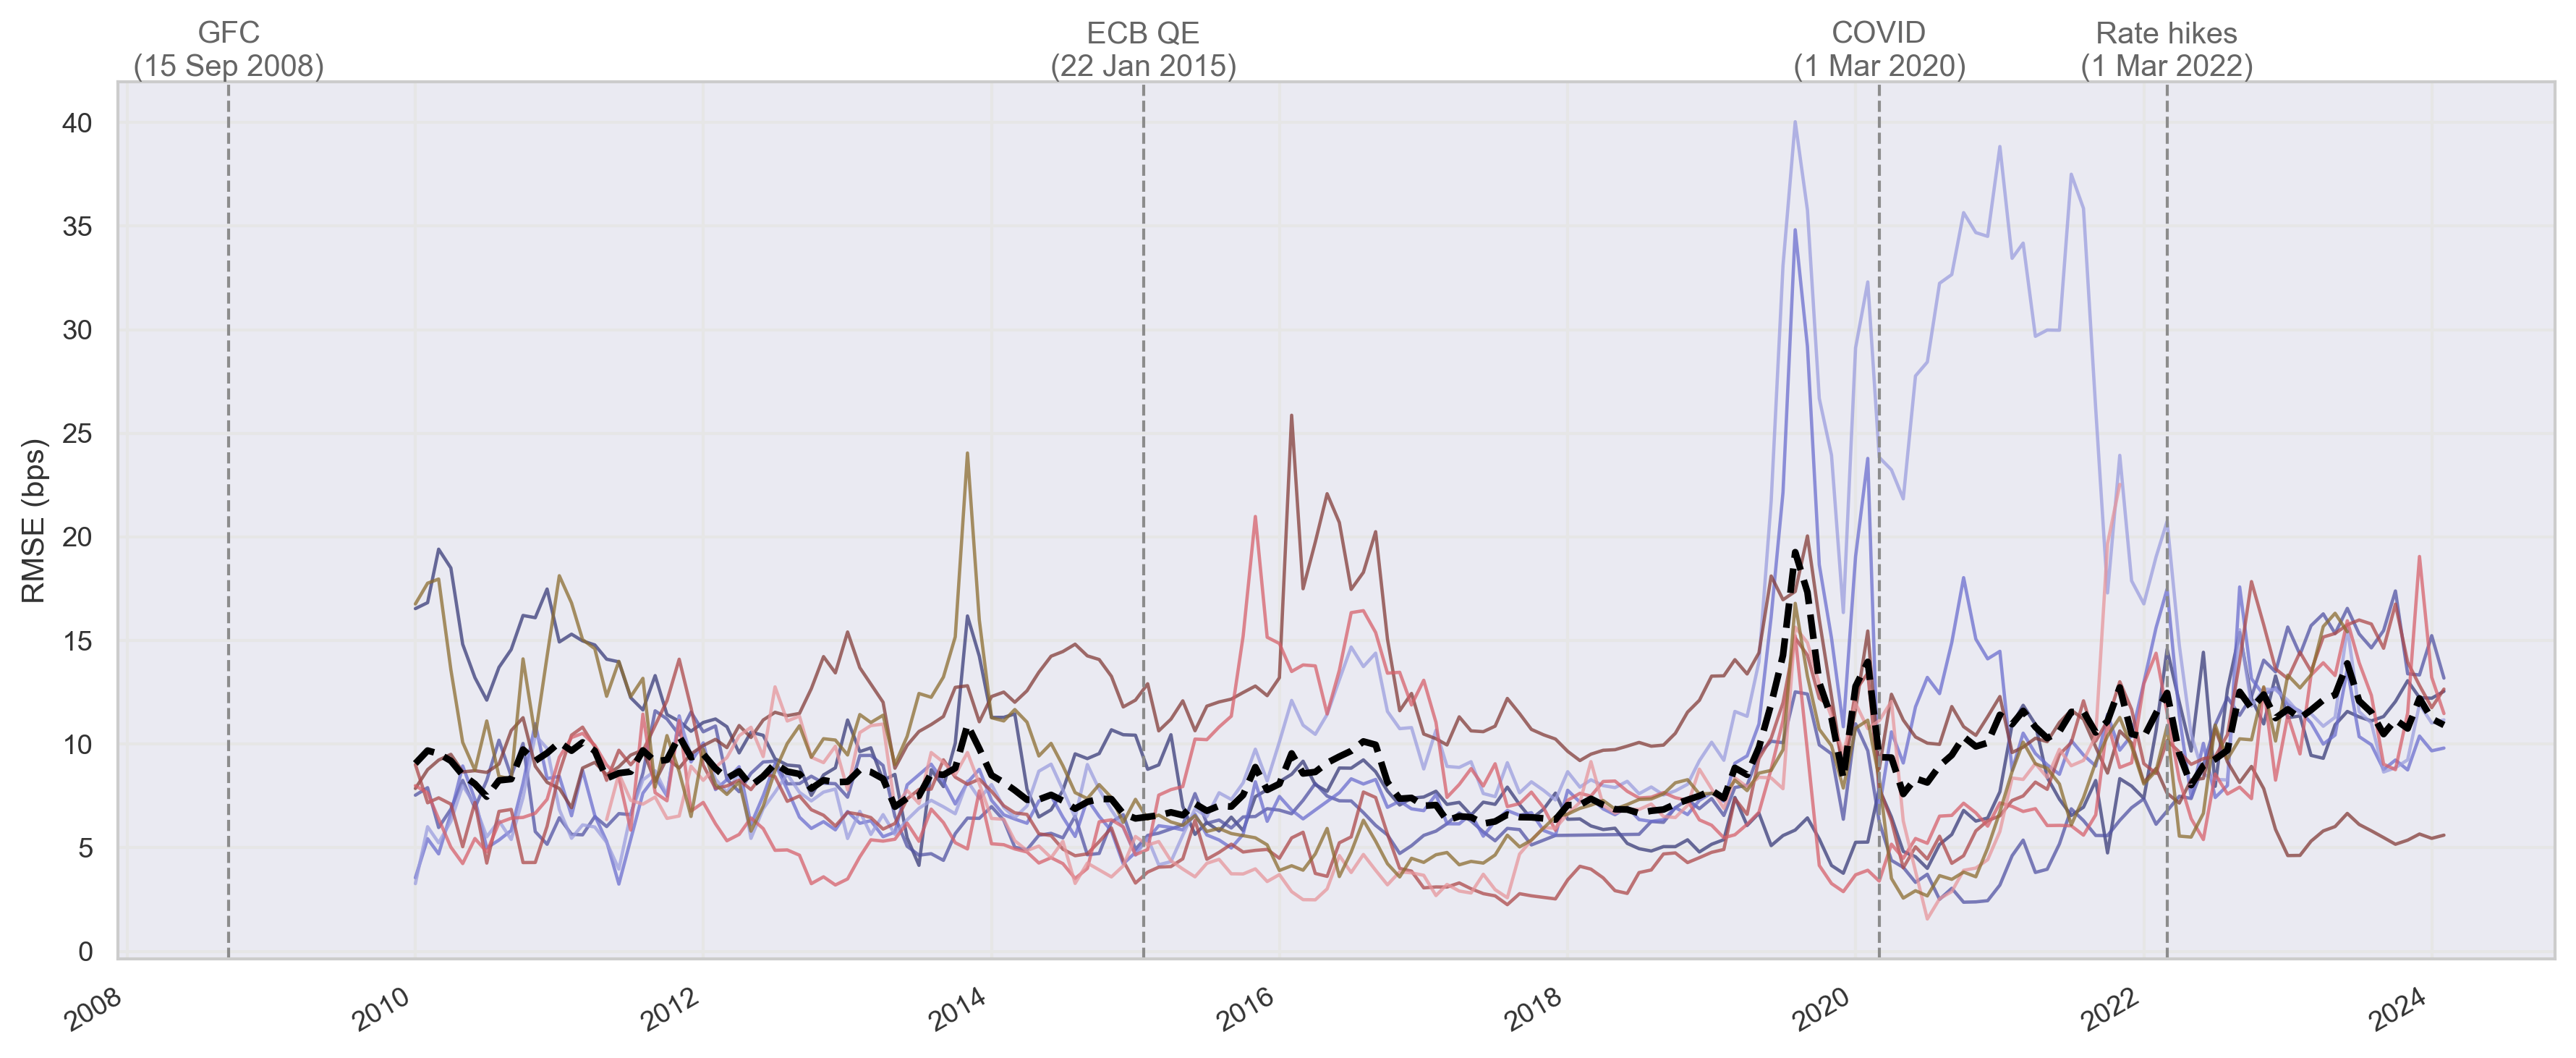
\includegraphics[width=0.85\textwidth]{Figures/thesis_results/AutoencoderPerformance/Q6b_rmse_over_time.png}
    \caption{In-sample RMSE (bps) over time for $\ell=3$,
    averaged across currencies per date.}
    \label{fig:Q6b}
\end{figure}

\begin{table}[H]
\centering
\caption{Top 10 worst in-sample fits ranked by RMSE (bps), $\ell=3$.
Per-tenor residuals shown in bps (fitted $-$ actual).}
\label{tab:Q6c}
\resizebox{\textwidth}{!}{%
\begin{tabular}{rlrrrrrrrrrr}
\toprule
Rank & Date & CCY & RMSE & 1Y & 2Y & 3Y & 5Y & 10Y & 15Y & 20Y & 30Y \\
\midrule
1  & 2016-11-30 & SEK & 5216.4 & $-$1809.2 & $-$9957.8 & $-$9974.4 & $-$3572.0 & $-$1279.6 & $-$839.5 & $-$655.1 & $-$484.0 \\
2  & 2016-02-29 & SEK & 5204.7 & $-$1796.7 & $-$9956.9 & $-$9975.5 & $-$3444.9 & $-$1267.0 & $-$836.6 & $-$652.9 & $-$483.6 \\
3  & 2016-10-31 & SEK & 5194.1 & $-$1299.9 & $-$9948.4 & $-$9964.7 & $-$3594.6 & $-$1279.3 & $-$830.4 & $-$640.7 & $-$465.7 \\
4  & 2015-11-30 & SEK & 5172.1 & $-$1978.0 & $-$9972.3 & $-$9992.5 & $-$2828.0 & $-$1192.0 & $-$822.0 & $-$663.6 & $-$507.7 \\
5  & 2016-03-31 & SEK & 5170.4 & $-$1744.3 & $-$9965.7 & $-$9983.5 & $-$3005.4 & $-$1214.2 & $-$821.0 & $-$649.7 & $-$487.8 \\
6  & 2016-12-30 & SEK & 5168.4 & $-$1716.6 & $-$9965.9 & $-$9985.0 & $-$2989.8 & $-$1211.0 & $-$818.1 & $-$647.8 & $-$485.4 \\
7  & 2017-01-31 & SEK & 5165.7 & $-$1912.2 & $-$9973.2 & $-$9995.3 & $-$2773.4 & $-$1188.3 & $-$818.3 & $-$655.5 & $-$498.8 \\
8  & 2016-04-29 & SEK & 5161.0 & $-$1776.7 & $-$9971.0 & $-$9990.6 & $-$2815.5 & $-$1195.4 & $-$816.0 & $-$652.0 & $-$497.8 \\
9  & 2016-05-31 & SEK & 5160.8 & $-$1653.2 & $-$9966.7 & $-$9985.4 & $-$2920.0 & $-$1205.6 & $-$814.0 & $-$645.0 & $-$486.9 \\
10 & 2017-02-28 & SEK & 5160.6 & $-$1612.9 & $-$9967.9 & $-$9986.0 & $-$2934.6 & $-$1204.5 & $-$814.7 & $-$645.3 & $-$483.7 \\
\bottomrule
\end{tabular}}
\end{table}


% Q6d
\begin{figure}[H]
    \centering
    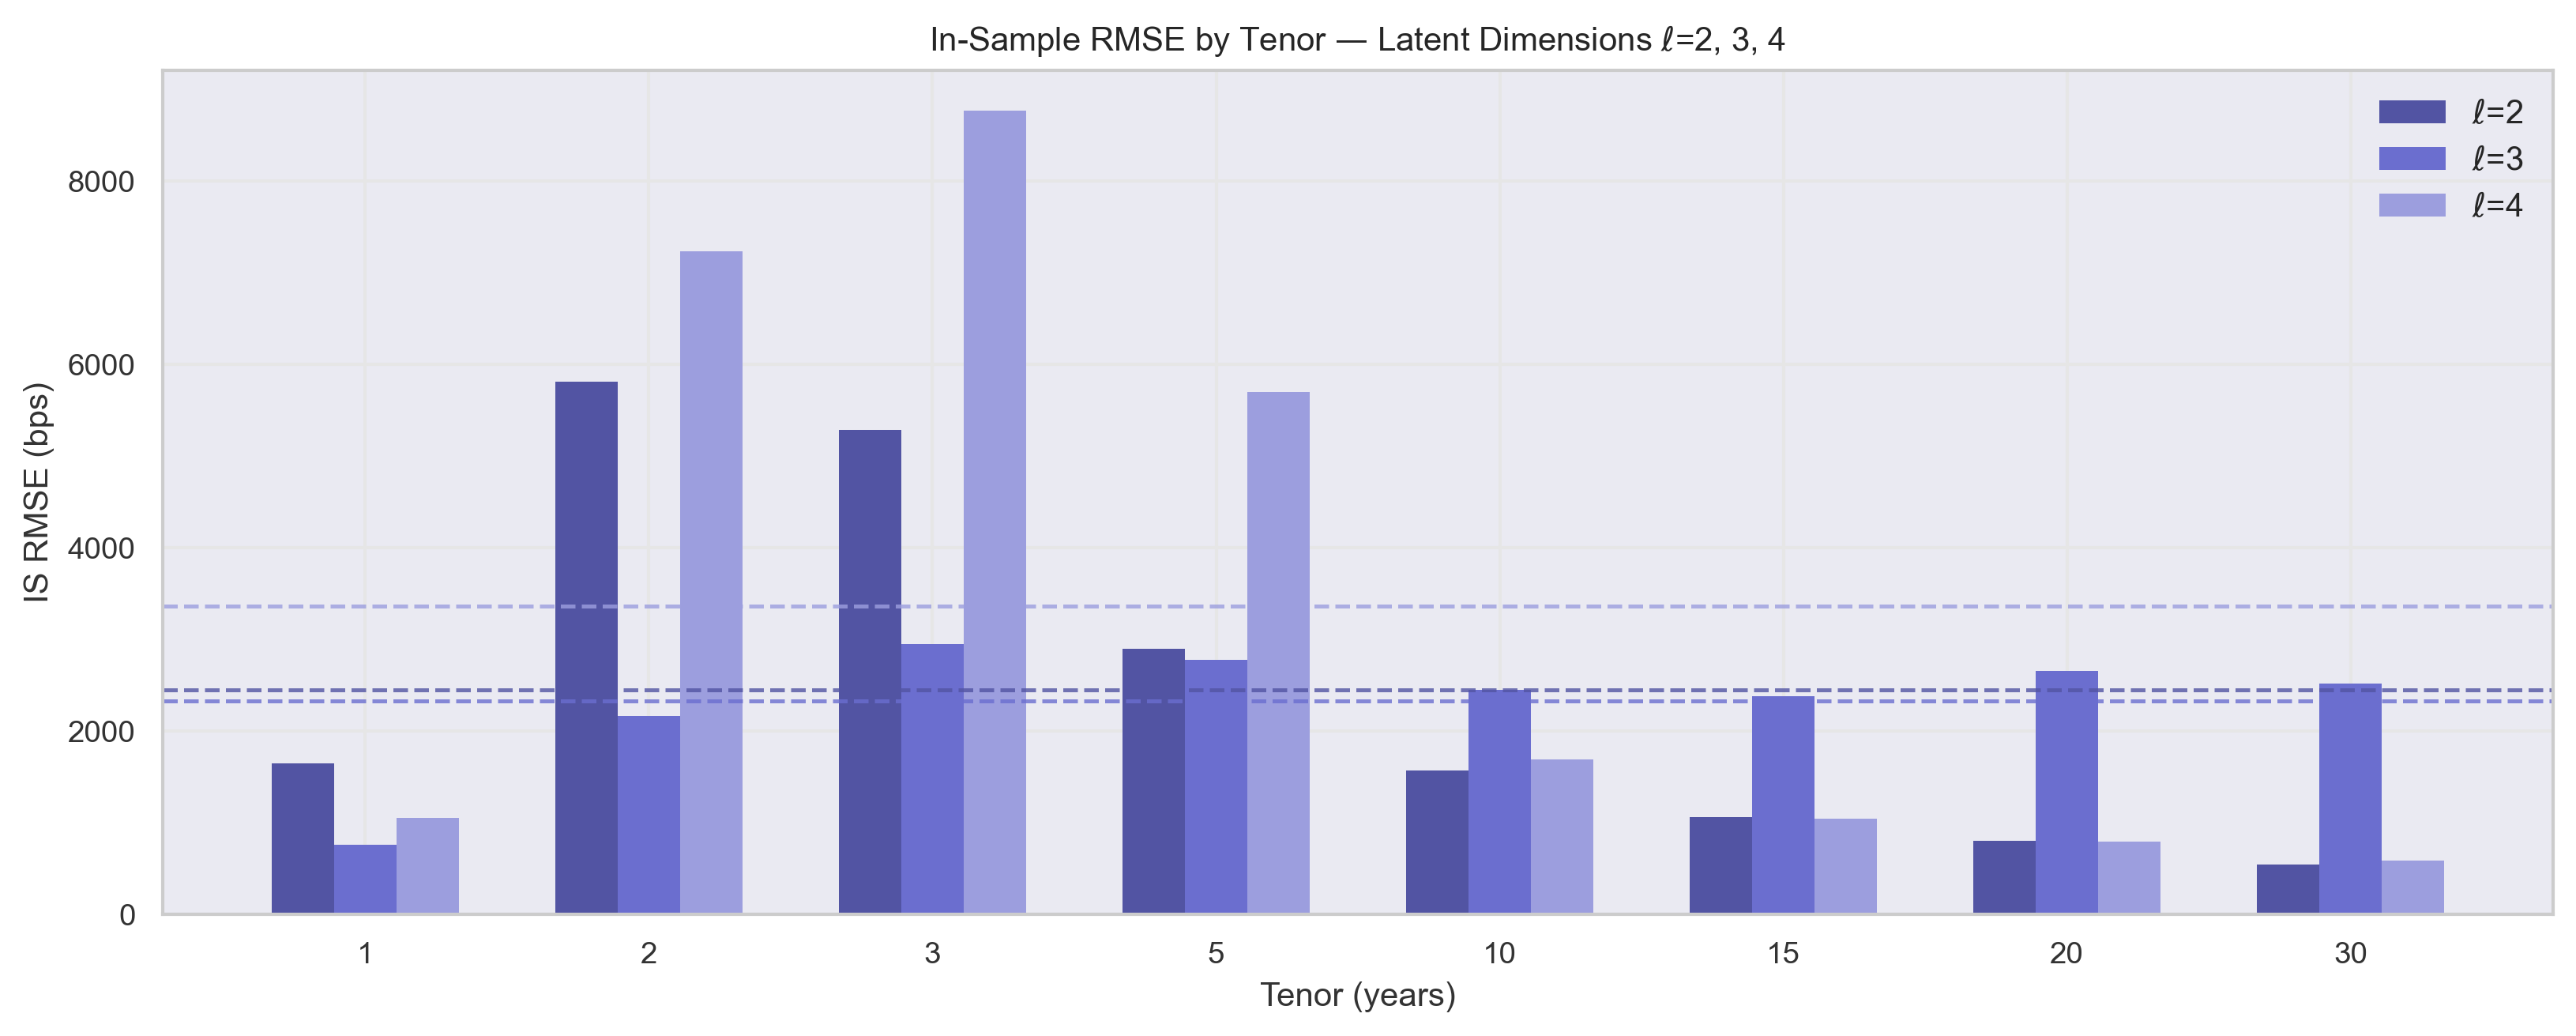
\includegraphics[width=0.85\textwidth]{Figures/thesis_results/AutoencoderPerformance/Q6d_rmse_by_tenor_all_dims.png}
    \caption{In-sample RMSE (bps) by tenor for latent dimensions
    $\ell=2,3,4$, averaged across currencies and dates.}
    \label{fig:Q6d}
\end{figure}

% ─────────────────────────────────────────────────────────────
\section{Question 7}
% ─────────────────────────────────────────────────────────────

\begin{figure}[H]
    \centering
    \begin{subfigure}{0.48\textwidth}
        \centering
        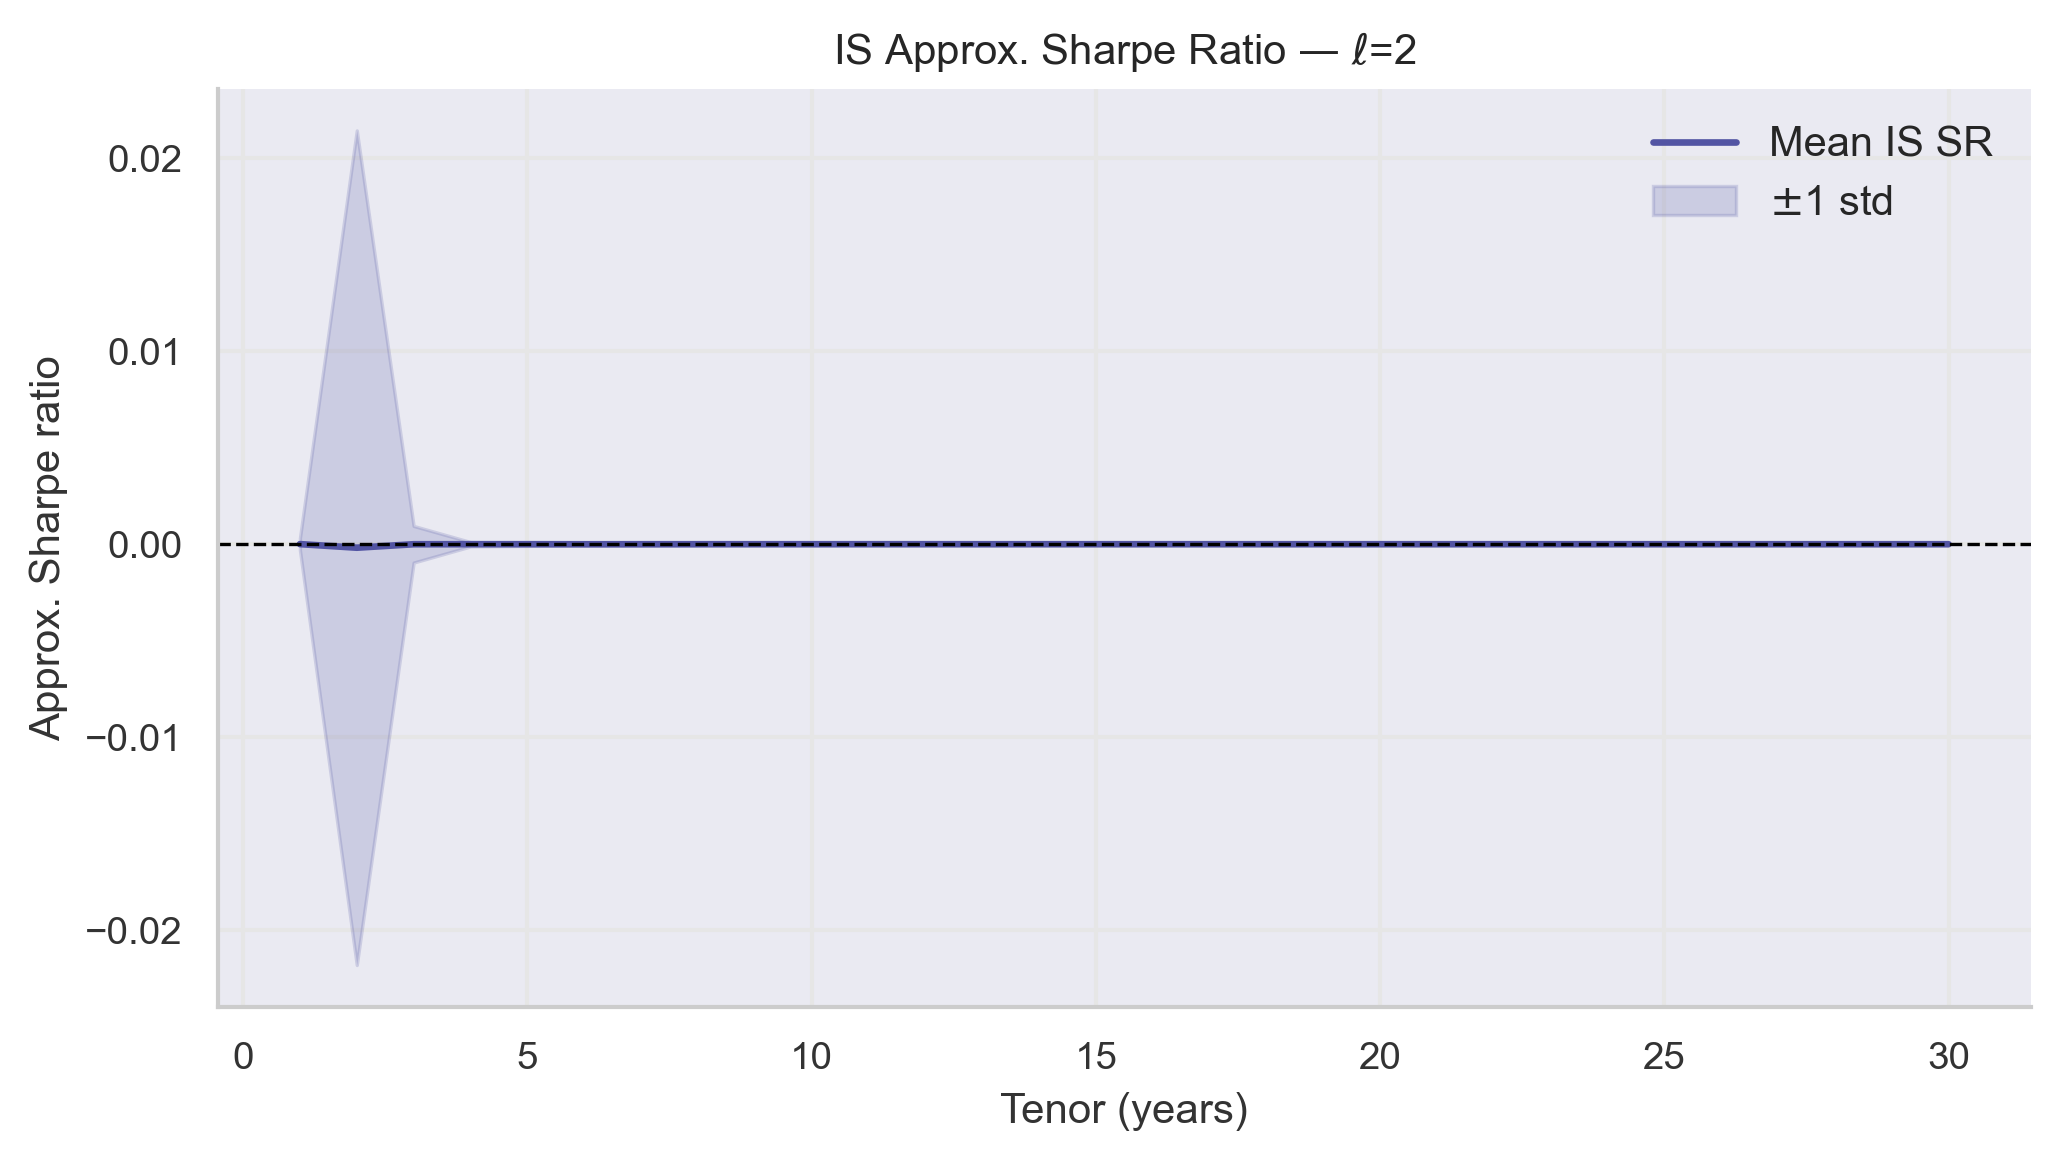
\includegraphics[width=\textwidth]{Figures/thesis_results/AutoencoderPerformance/Q7_sharpe_ratio_IS_dim2.png}
        \caption{AE $(\ell=2)$}
    \end{subfigure}
    \hfill
    \begin{subfigure}{0.48\textwidth}
        \centering
        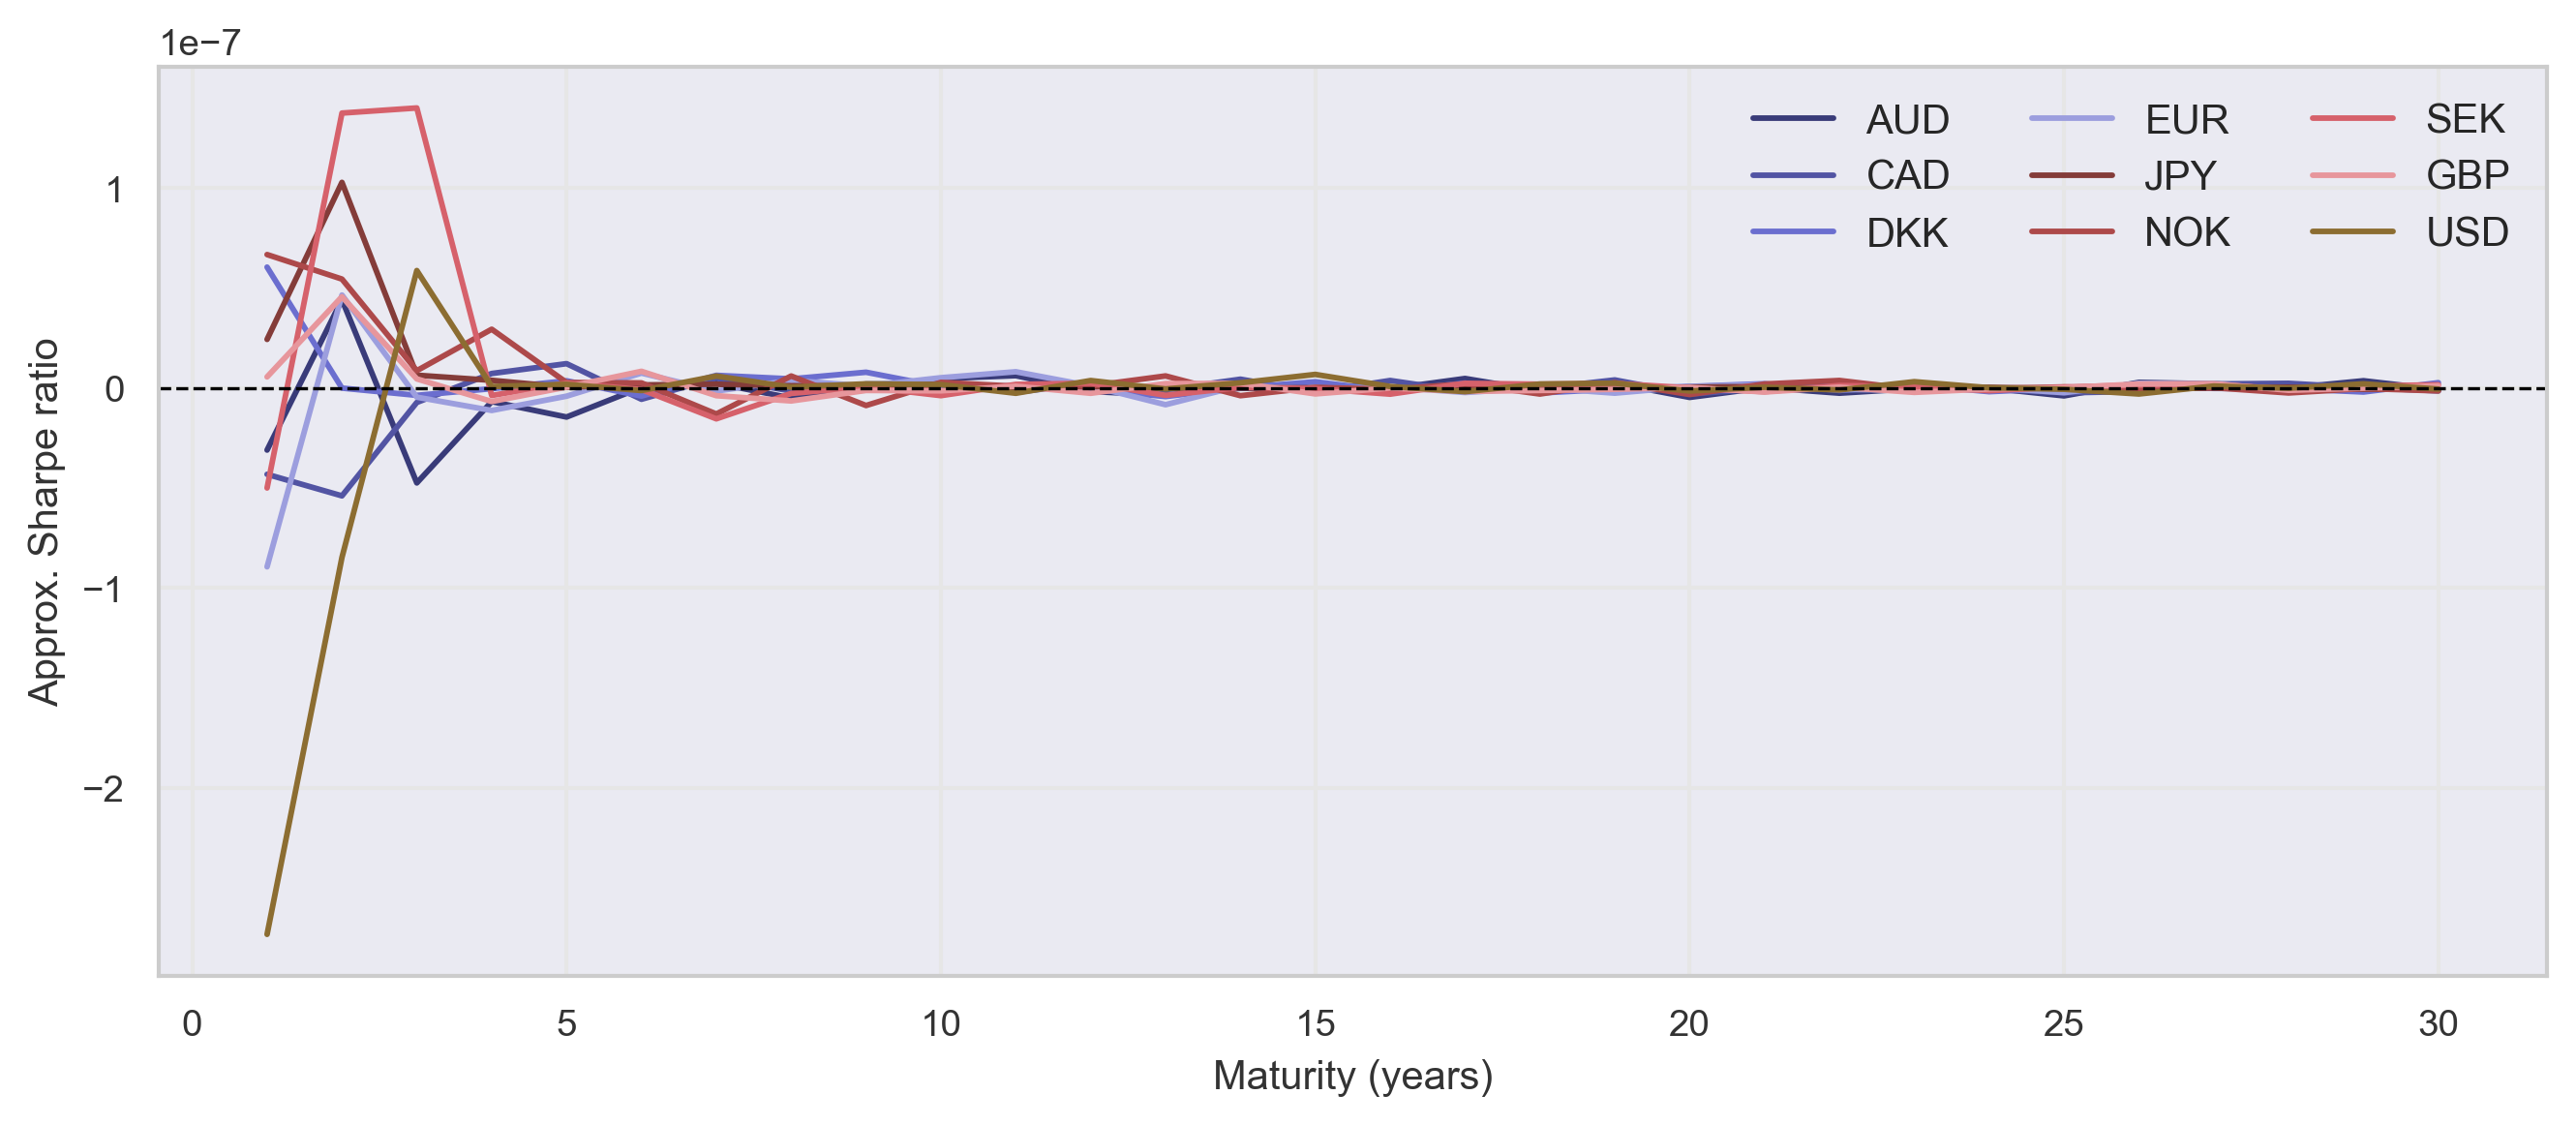
\includegraphics[width=\textwidth]{Figures/thesis_results/AutoencoderPerformance/Q7_sharpe_ratio_IS_dim3.png}
        \caption{AE $(\ell=3)$}
    \end{subfigure}

    \vspace{0.25cm}

    \begin{subfigure}{0.48\textwidth}
        \centering
        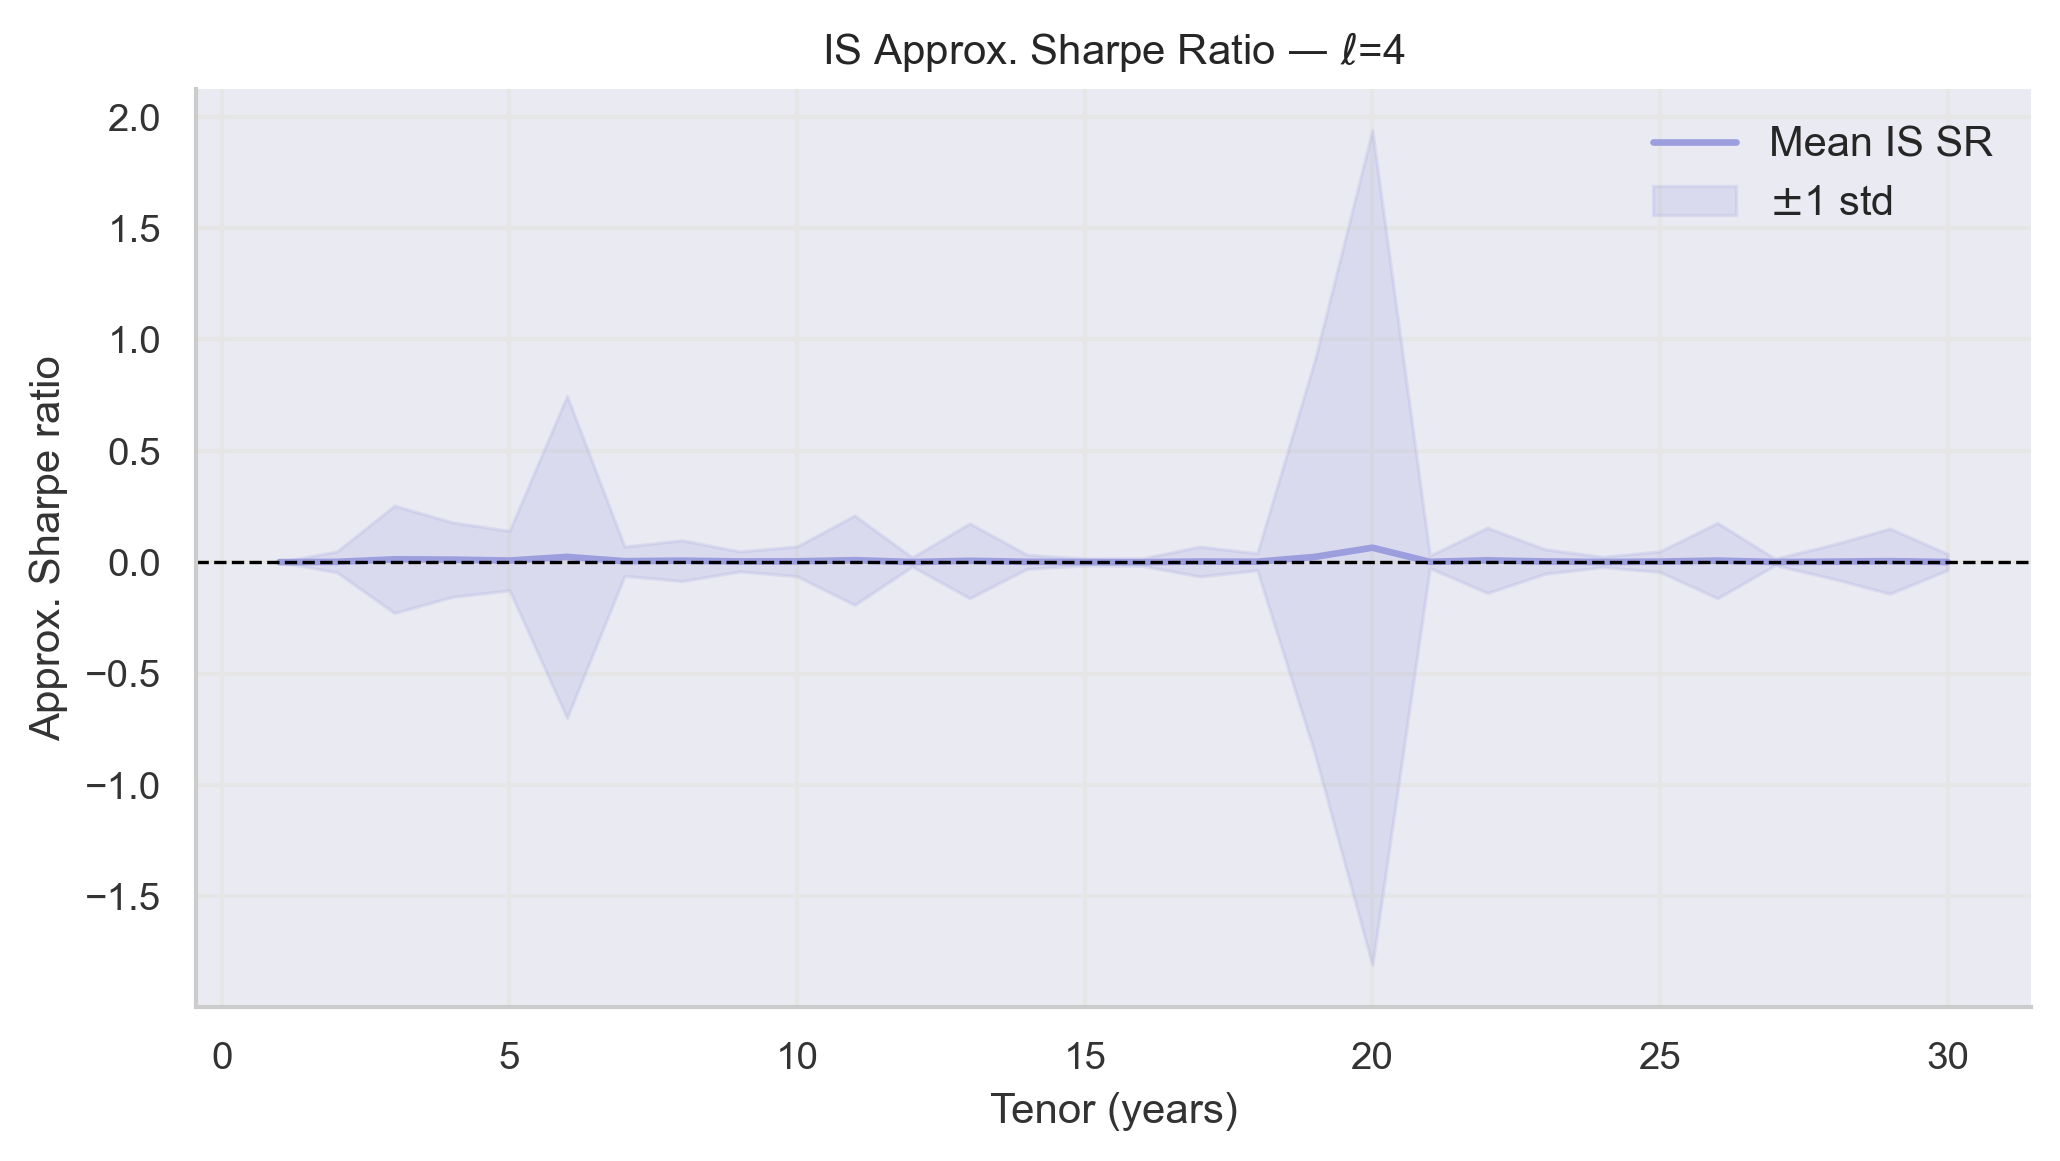
\includegraphics[width=\textwidth]{Figures/thesis_results/AutoencoderPerformance/Q7_sharpe_ratio_IS_dim4.png}
        \caption{AE $(\ell=4)$}
    \end{subfigure}

    \caption{In-sample approximate Sharpe ratio across tenors (1--30Y)
    for $\ell=2,3,4$. Shaded band shows $\pm$1 standard deviation
    across training observations. Dashed line marks zero (no-arbitrage reference).}
    \label{fig:Q7_sharpe}
\end{figure}




